\chapter{Background Information and Related Work}

In the following chapter, we further explore the motivation for undertaking the project,
analyse the current state of the project domain and outline the research that will form the basis for the rest of the report.

\section{The Problem}

As previously mentioned, the goal of this project is to automate the feature selection process for a website fingerprinting attack.
By this we mean that given a specific trace, our model should be able to produce a fixed-length vector that is a close representation of the respective trace.
However, before we delve into the details of the attack, we first need to gain a greater understanding of some concepts such as
onion routing, website fingerprinting deep learning.

\subsection{Onion Routing}

To preserve privacy, we do not only need to obscure the content of a web page but also hide who is taking to whom \cite{goldschlag1999onion}.
Tor achieves both of these by making use of a technique, called \textit{onion routing}, which is a simple protocol that can be divided up into three phases:
\textit{connection setup}, \textit{data movement} and \textit{connection tear-down} \cite{goldschlag1999onion}.
We show how the protocol works by providing a simple example of Alice trying to communicate with Bob.

\begin{enumerate}
  \item \textbf{Connection Setup:}
    \begin{itemize}
      \item Alice's Tor client obtains a list of Tor nodes from a directory server.
      \item From these, Alice picks three random Tor nodes and labels them \textit{one, two} and \textit{three}.
      \item Alice communicates with the first node and shares a symmetric key.
      \item From now on, all the messages that Alice will send will be encrypted and sent to the first node and forwarded from there onwards.
        Including the messages to share a symmetric key with the second node, such that the second node does not know Alice's true identity.
        Instead, it just knows that the messages are coming from the first node.
      \item Again, now all messages are first sent to the first node and forwarded to the second node, which it in turn forwards to the third and final node.
        This way, Alice shares the final symmetric key with the third node.
    \end{itemize}

    What is important here is that we use a secure key-sharing algorithm such that only Alice and the respective node know the keys.
    Additionally, since all of the traffic is forwarded from the first node, the second and the third nodes do not know the true identity of Alice.

    \begin{figure}[ht]
      \centering
      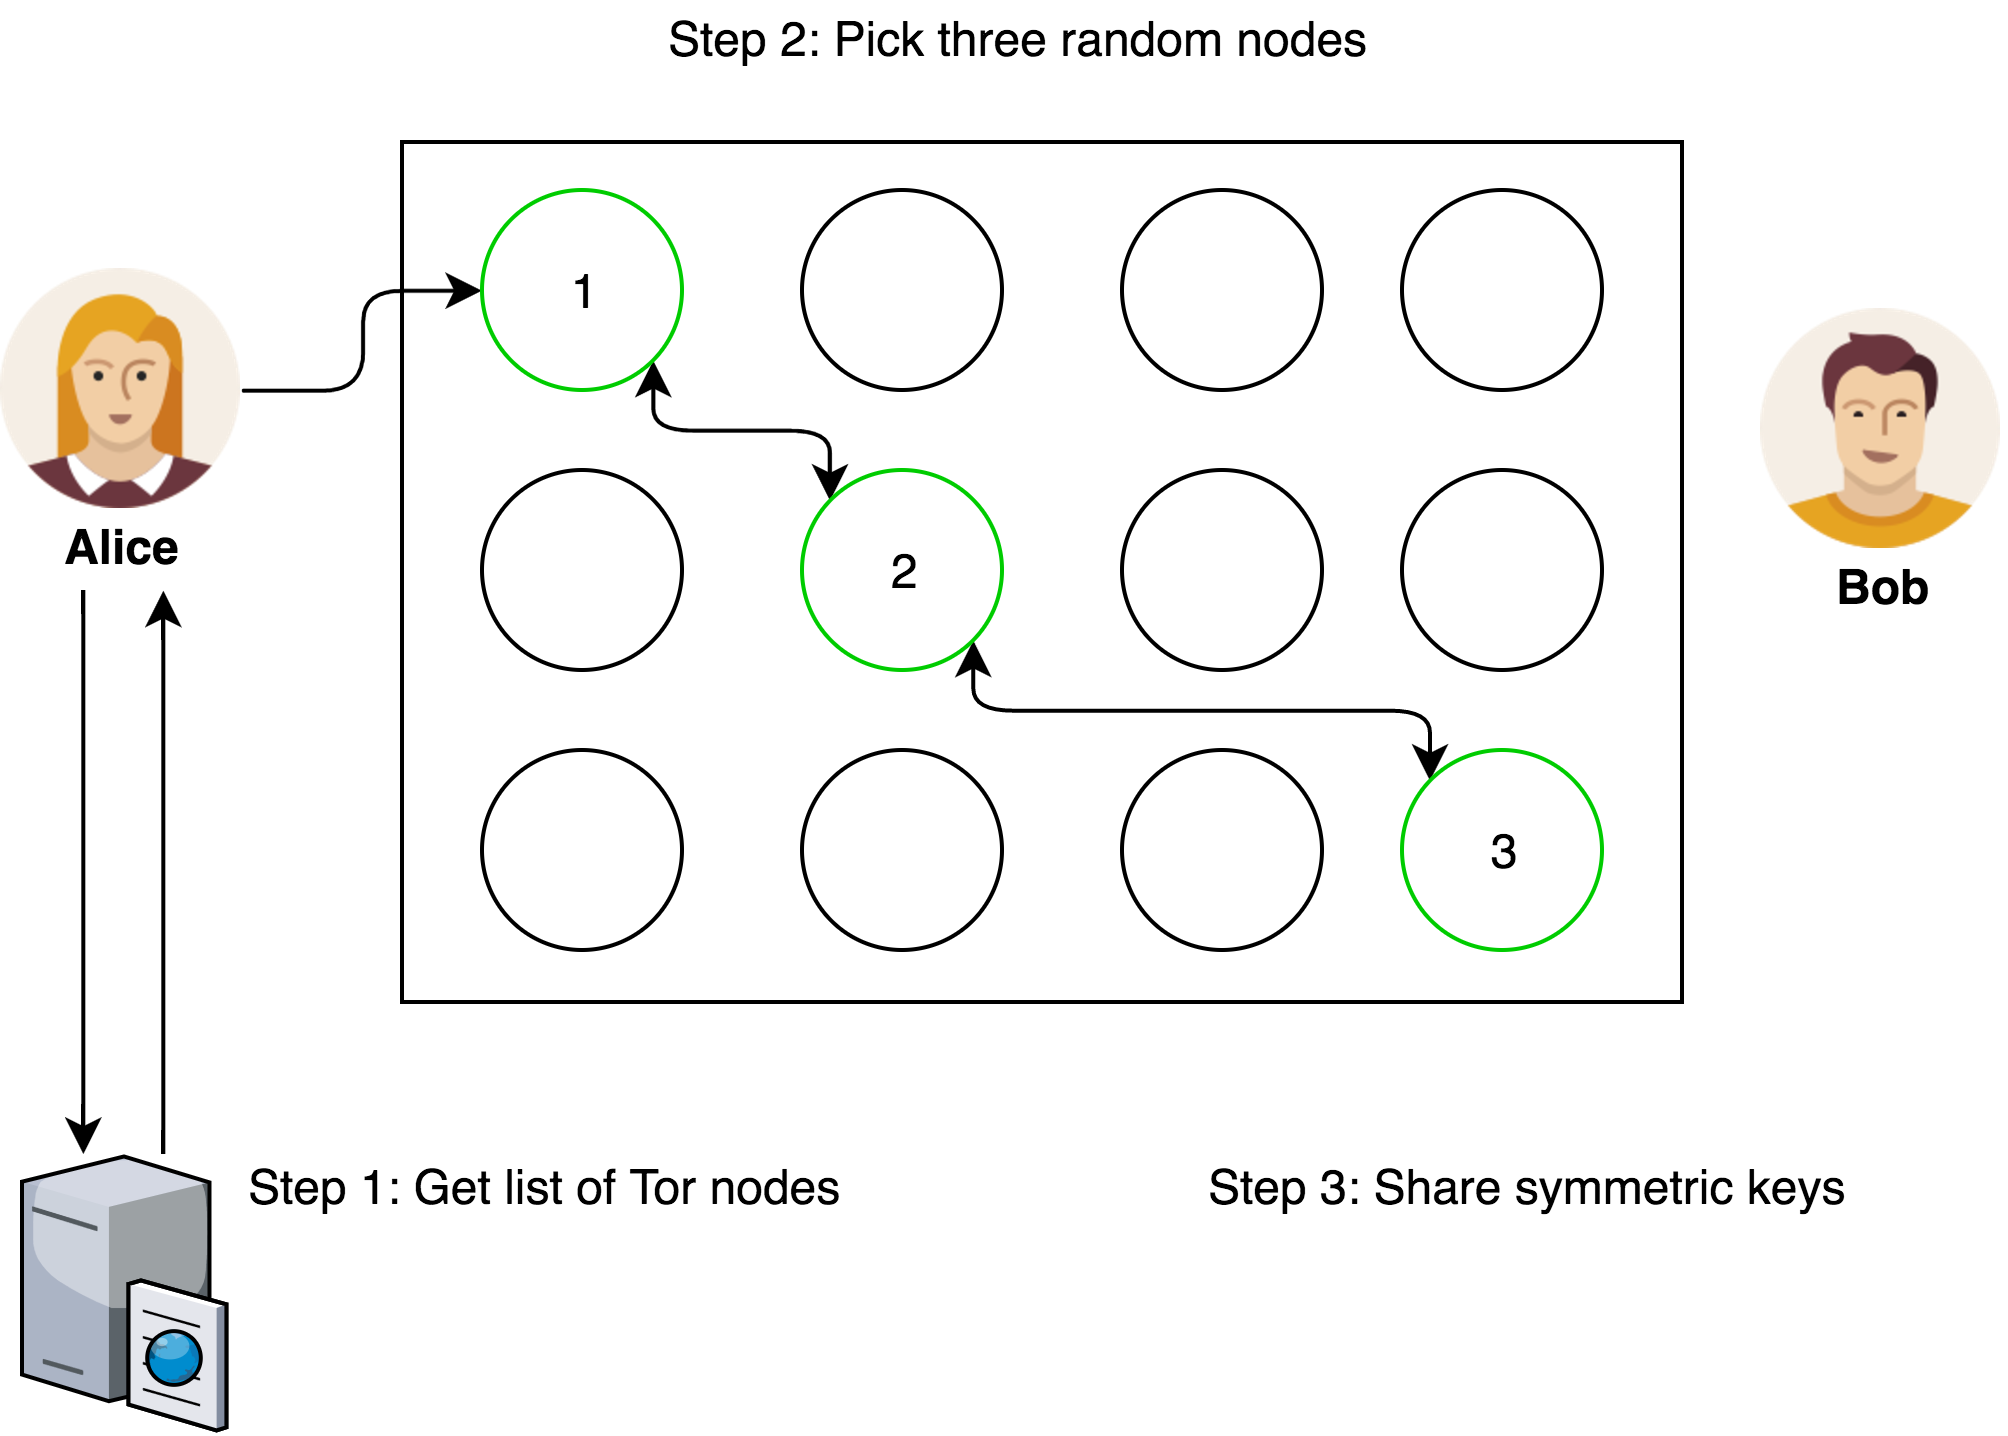
\includegraphics[width=0.6\textwidth]{tor_setup}
      \caption{An example of a connection setup for the onion routing protocol.}
      \label{fig:tor_setup}
    \end{figure}

  \newpage

  \item \textbf{Data Movement:}
    \begin{itemize}
      \item Before Alice can send any data, she first needs to encrypt it in different layers. By this we mean that first it encrypts the data \textit{(adressed to Bob)}
        using the shared key from the third node and addresses that encrypted data to the third node.
        Next, she encrypts that data again using the key from the second node and addresses it to the second node.
        Finally, as expected, it encrypts the data a final time using the shared key from the first node.

      \item Now Alice is ready to send the data to the first node.
      \item Once the first node received the data, it decrypts it using the shared key. This reveals the address to the second node.
        The key is here that the first node cannot see the data nor can it see Bob's address, since that information is still encrypted.

      \item Next, the first node forwards the data, it just decrypted, to the second node.
        Again, this node decrypts the data, revealing the address to the third node
        but now it doesn't know what the data is, where the final destination is or where it originally came from.

      \item Lastly, the second node forwards the data to the third node. After decryption, this final node can see the data and where it is going but it does not know where it originally came from.
        So it forwards the data to Bob and none of the nodes know all of the following: the data, the final destination or where it originally came from.
    \end{itemize}

    The protocol is called onion routing because it encrypts the data in multiple layers and at every node, one of the layers of the onion is peeled off \cite{tor_project2}.
    The key is that none of the nodes know the complete path that has been taken.

    \begin{figure}[ht]
      \centering
      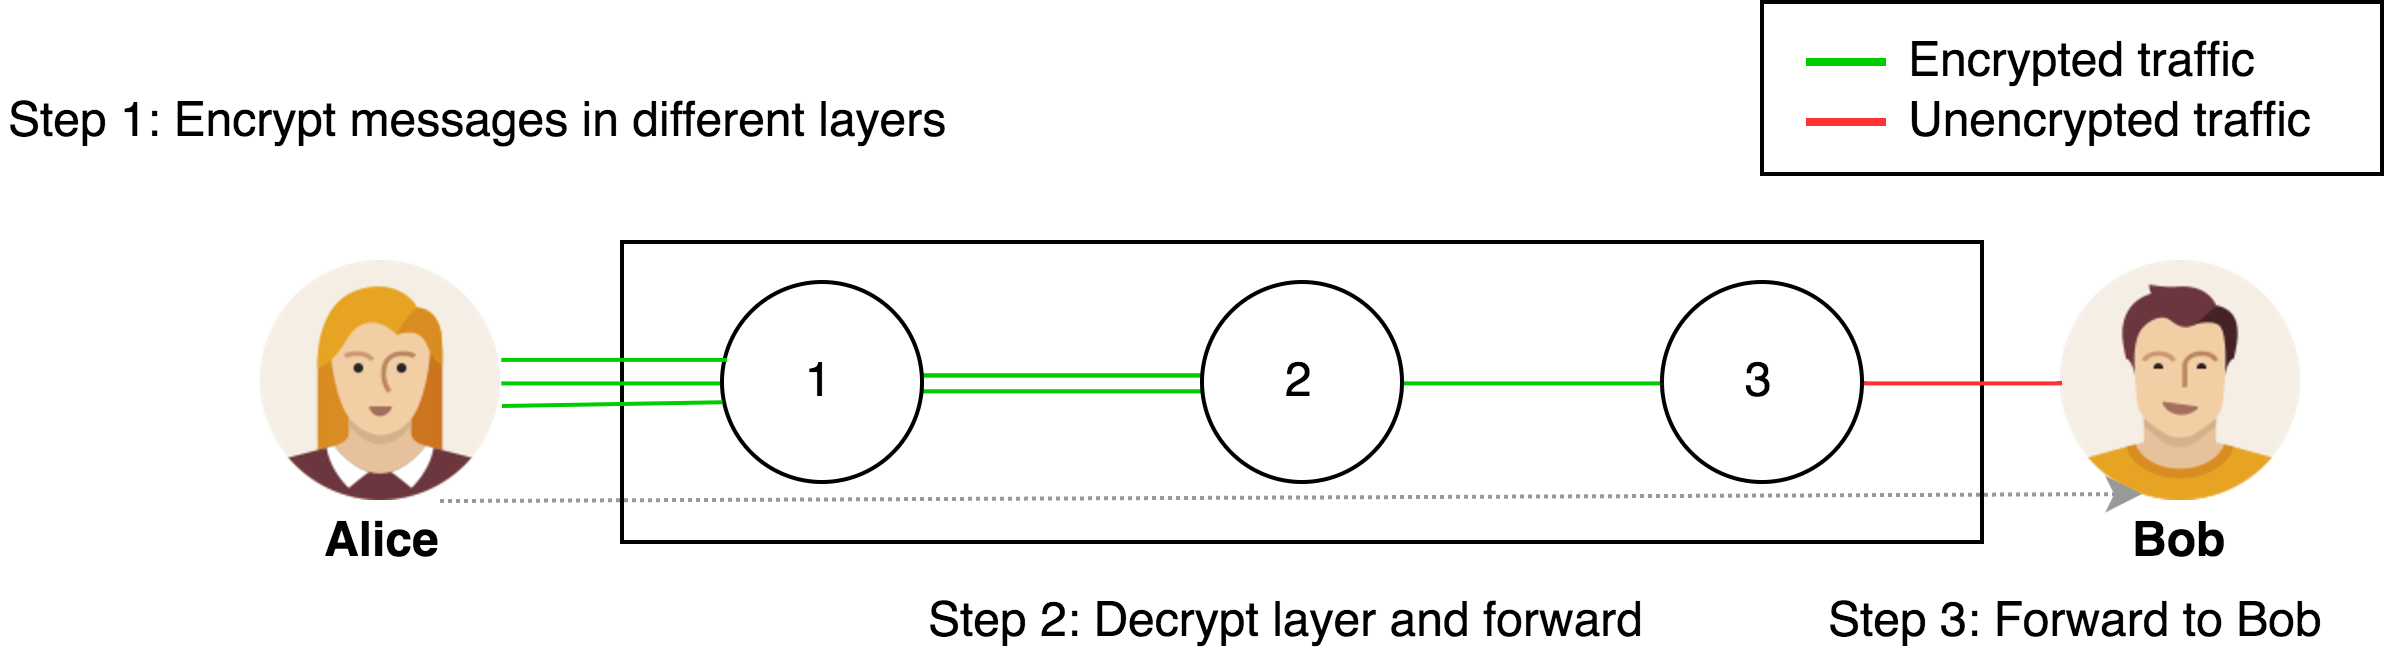
\includegraphics[width=0.75\textwidth]{tor_message_sending}
      \caption{Sending a message with the onion routing protocol.}
      \label{fig:tor_message_sending}
    \end{figure}

  \item \textbf{Connection Tear-down:} This can be initiated by any of the nodes or the client and the process is straightforward.
    Either the client sends a request for a tear-down to the first node to remove any data on the connection (including the shared key), which is then forwarded to the other nodes.
    Or one of the nodes sends a tear-down message to both the previous node and the next node, which are then forwarded in both directions \cite{goldschlag1999onion}.

\end{enumerate}

Tor generally uses the same circuit for connections that happen within around 10 minutes after creating a circuit.
Later requests, however, are given a new circuit \cite{tor_project, tor_project2}.

\section{Related Work}

\subsection{Website Fingerprinting} \label{sec:related-work}

Website fingerprinting (WF) is the process of a \textit{local} adversary attempting to identify which web pages a specific client visits by analysing their traffic traces.
By this we mean that the attacker can eavesdrop on the traffic between the client and the first Tor node (or \textit{entry node}), as shown in figure \ref{fig:threat_model}.
So it can be anyone from a person on the same network to an ISP.
The reason as to why the attacker has to be local is because in onion routing systems, it is the only place in the network where you still know
the true identity of the client.

\begin{figure}[ht]
  \centering
  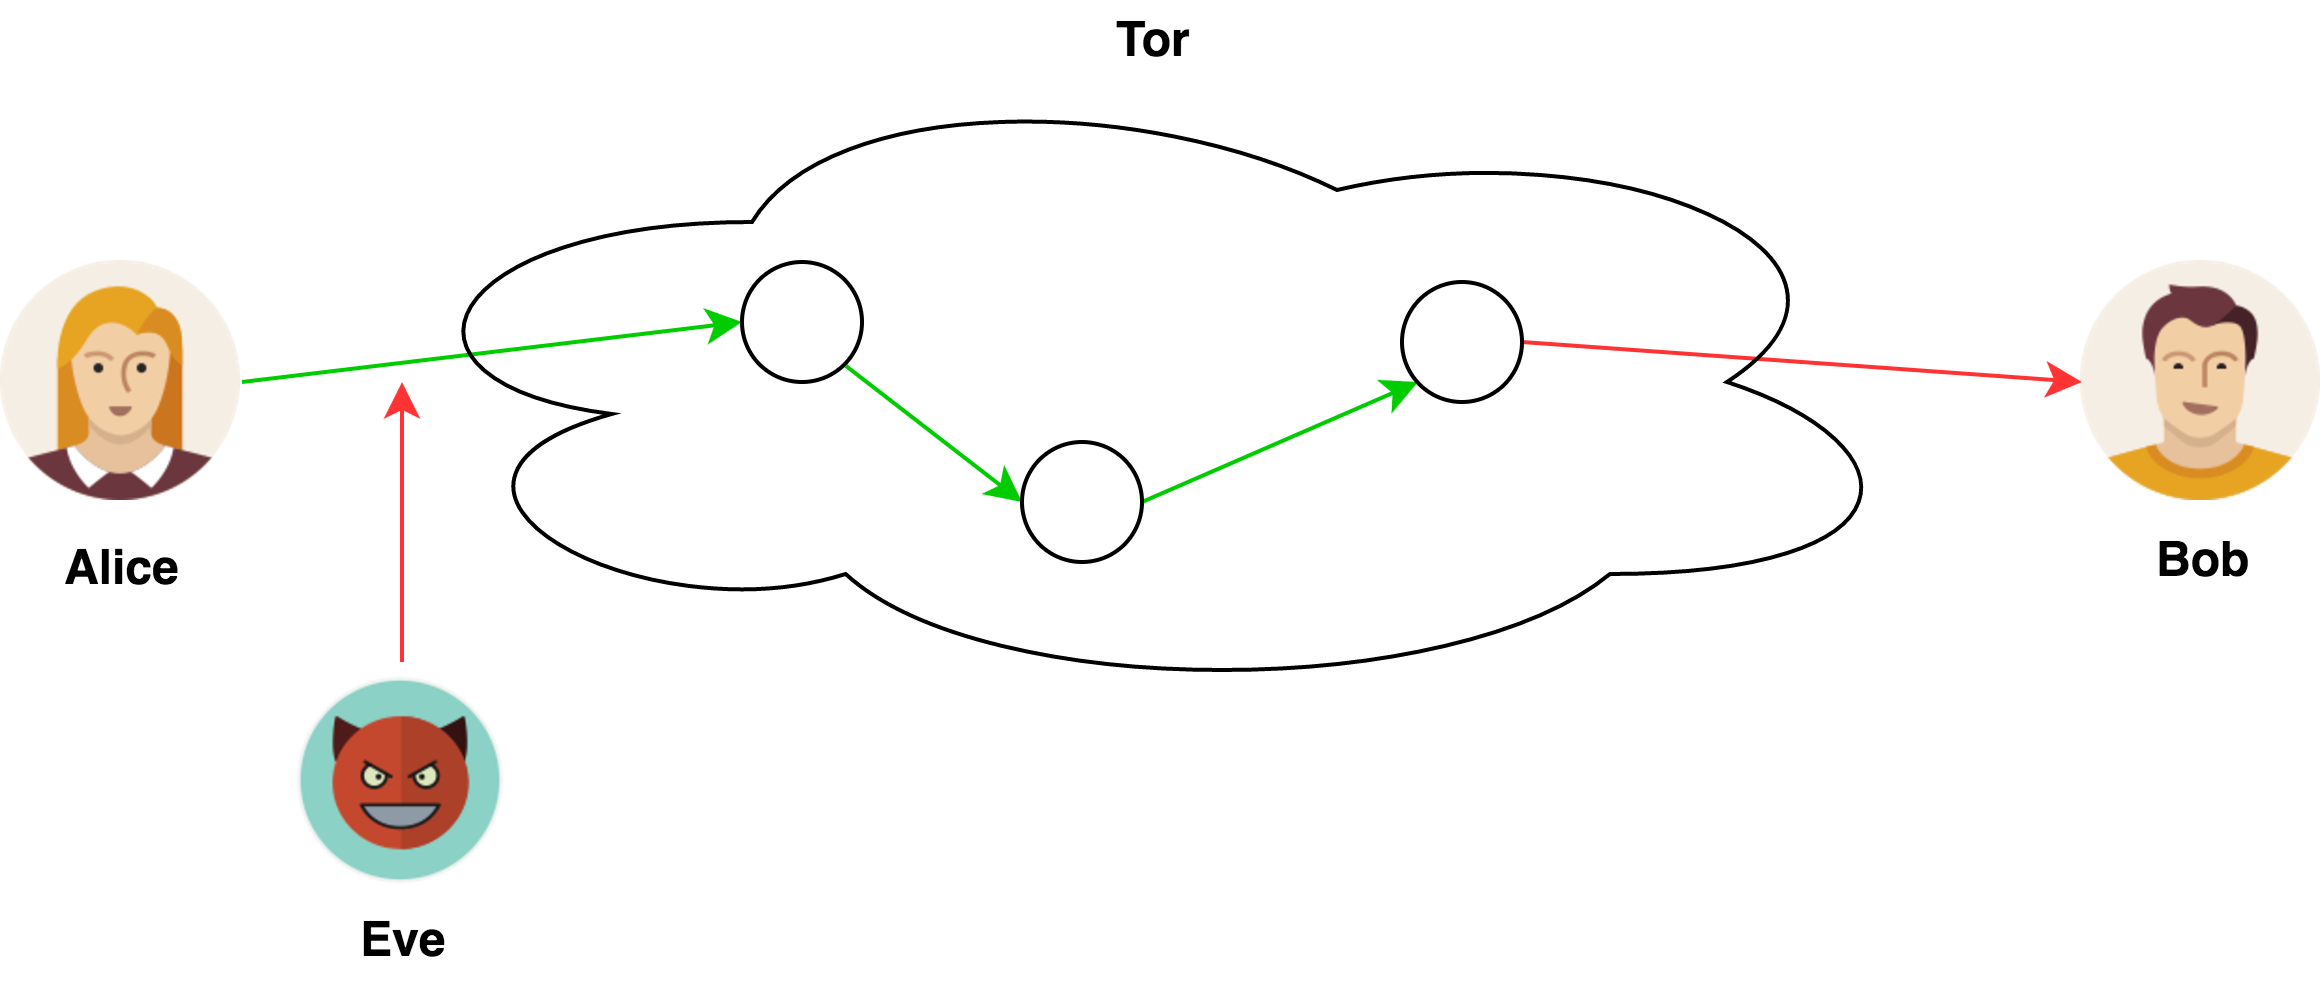
\includegraphics[width=0.75\textwidth]{threat_model}
  \caption{Threat model for a simple website fingerprinting attack.}
  \label{fig:threat_model}
\end{figure}

In general, the attack is as follows. The attacker first collects a dataset, containing packet traces for loading several web pages.
In practice, these web pages are the ones that an attacker is interested in monitoring and a small amount of unmonitored pages as noise.
From those traces, the attacker extracts a fixed number of features, the so-called \textit{fingerprint}.
Next, it uses those fingerprints to train some sort of model \textit{(often a machine learning model)} to find patterns in the data.
Finally, the adversary observes packet traces, generated by the client, and uses the previously trained model to classify which web pages the user is visiting.
Therefore, an attack is essentially a classification problem, where you try to map packet traces into web pages.

We should denote that throughout this report, we will be using the term ``web pages'' rather than ``websites''.
The reasoning behind this is that a website often consists of multiple web pages,
which can result in significantly different traffic traces, depending on which document you load.

The term \textit{``website fingerprinting''} was first mentioned by A. Hintz who performed a simple traffic analysis on Safeweb,
an encrypting web proxy that tried to protect user's privacy \cite{hintz2002fingerprinting}. Although the attack was simple, it and other earlier
works show the possibility that encrypted channels might still leak information about the URL \cite{hintz2002fingerprinting, wagner1996analysis}.
Later, in 2009, the first fingerprinting attack against Tor was executed by Herrmann et al. using a \textit{multinomial naive bayes} model.
They managed to get a relatively high accuracy for several protocols, such as \textit{OpenSSL} and \textit{OpenVPN}, on a small set of 775 web pages.
However, on more specialised anonymization networks such as Tor, the model only achieved a 2.96\%, which they claim was caused by a suboptimal configuration \cite{herrmann2009website}.

Around the same period Y. Shi et al. performed an attack that specifically focused on anonymity systems such as Tor \cite{shi2009fingerprinting}.
Using a \textit{cosine similarity}, they achieved around 50\% accuracy on an even smaller dataset of only 20 web pages \cite{shi2009fingerprinting}.
The first real threat however, was by A. Panchenko et al. who used a \textit{support vector classifier} (SVC) on the same dataset of 775 web pages as Herrmann et al.
and got a 54.61\% success rate \cite{herrmann2009website, panchenko1}.

All of the previously mentioned research, except the one done by Panchenko et al. have only considered a \textit{closed-world scenario}.
A closed-world setting means that all of the web pages are known in advance \cite{panchenko1}.
For instance, when Herrmann et al. trained their model on a dataset of 775 web pages, they made the assumption that a client could only visit one of
those web pages and none other.
In an \textit{open-world scenario}, however, the attacker does not know in advance which URLs the victim might visit.
The most prominent example of this is when the authorities want to monitor which people try to access a set of censored sites \cite{panchenko1}.
In order to achieve this, the models need to be trained on both \textit{monitored} and \textit{unmonited web pages}.

Wang et al. later conducted an attack on Tor using a novel \textit{k-nearest neighbor} (k-NN) classifier with \textit{weight adjustment} on a large feature set (3736 features).
In addition to getting around 90\% accuracy, they also significantly reduced the time needed for training \cite{wang_cai_johnson_nithyanand_goldberg_2014}.

Next, using a completely different approach, Hayes et al. extracted fingerprints using a \textit{random forest} \cite{kfingerprinting}.
This novel technique involved storing a \textit{fingerprint} as a set of leaves within that forest.
Next, they simply use the \textit{hamming distance} as a distance metric to find the k-nearest neighbors.
If all the labels within those $k$ instances are the same, the model classifies the new instance as the previously mentioned label and as an unmonitored page otherwise.
The interesting aspect is that changing the value of $k$ allows them to vary the number of \textit{true positives} (TP) and \textit{false positives} (FP) \cite{kfingerprinting}.

Finally, Panchenko et al. improved upon their previous attack to create one of the current state-of-the-art methods.
They tested their approach on several datasets, including the one used by Wang et al. in their k-NN attack, where they got around 92\% accuracy.
In an open-world scenario, on the other hand, they claim to have gotten up to 96\% accuracy.

\subsection{Automatic Feature Selection}

At the time of writing, there are not many works that have examined the use of automatic feature selection techniques in the context of a website fingerprinting attacks.
First, Abe et al. study the use of a \textit{stacked autoencoder} with a \textit{softmax classifier} \cite{deeplearning}.
However, since a stacked autoencoder still requires a fixed-length input, they pad and truncate cells, whose length is shorter or longer than $5000$.
With it, they manage to achieve a $88\%$ accuracy \cite{deeplearning}.

V. Rimmer takes a similar approach, as she also uses a stacked autoencoder with a softmax classifier \cite{deeplearningthesis}.
But rather than padding or truncating the cells, she transforms the traces into a fixed-length histogram or \textit{wavelength coefficients}.
With this, she manages to achieve a $71\%$ accuracy.

\newpage

\subsection{Defenses} \label{sec:defenses}

Not only has there been research regarding different attacks but there are also various works that describe possible defenses.
First of all, Tor already implements \textit{padding}, which means that all packets are padded into fixed-sized cells of $512$ bytes.
Next, in response to the first attack by Panchenko et al., Tor also supported randomized ordering of HTTP pipelines \cite{panchenko1, kfingerprinting, perry2011experimental}.
Finally, on top of these defenses, fingerprinting on Tor is made more difficult by all of the background noise present.
This is due to the fact that Tor also sends packets for circuit construction and \textit{SENDME's}, which ensure flow control \cite{panchenko2}.
Although Wang et al. proposed a probabilistic method to remove these \cite{wang_goldberg_2013}, they still make the classification process slightly more difficult.

Next, Lua et al. designed an application-level defense, that was able to successfully defend against a number of classifiers by modifying packet size, timing of packets, web object size, and
flow size \cite{perry2011experimental}. This is achieved by splitting individual HTTP requests into multiple partial requests, using extra HTTP traffic as a cover and making use of HTTP pipelining \cite{cai_zhang_joshi_johnson_2012}.
Although this has been a relatively effective technique to obfuscate traffic, several attacks have proven that this defense only still does not suffice \cite{cai_zhang_joshi_johnson_2012,wang_cai_johnson_nithyanand_goldberg_2014}.

\textit{BuFLO}, on the other hand, is a \textit{simulatable} defense \cite{wang_cai_johnson_nithyanand_goldberg_2014}, designed by Dyer et al. that performs packet padding and sending data at a constant rate in both directions \cite{dyer2012peek}.
The disadvantage of this method is the high overhead required in order to keep the constant data rate.
Some extensions have been described that try to minimize this overhead such as  Nithyanand's work that uses existing knowledge of a website traces to maintain a high level of security \cite{nithyanand2014glove}.

More recently, Cherubin et al. developed the first website fingerprinting defense on the server side \cite{cherubin2017website}.
This can be particularly interesting for \textit{Tor hidden services} that want to provide all of their users the privacy that they require.
The attack uses a technique, called \textit{ALPaCA}, which pads the content of a web page and creates new content to conceal specific features on a network level \cite{cherubin2017website}.

Finally, there are also some other techniques such as \textit{decoy pages} and \textit{traffic morphing} \cite{wright2009traffic,panchenko1}.
Decoy pages, or sometimes called \textit{camouflage}, is a simple defense that involves loading another web page whenever a page is requested.
This process provides more background noise, which makes fingerprinting more difficult \cite{panchenko1}.
Traffic morphing, on the other hand, is a slightly more complex technique that changes certain features in the traffic in order to make it appear as if another page is loaded \cite{wright2009traffic}.

\subsection{Critical Analysis}

Most attacks, that have been described above, are based on a set of different assumptions.
Here we list these assumptions and analyze if they are reasonable.

The first assumption we examine are open and closed-world scenarios.
One of the main problems with website fingerprinting is the amount of web pages readily available on the web.
An open-world scenario tries to solve this issue by only classifying a small amount of web pages and by labelling the other ones as unmonitored.
However, machine learning theory states that the bigger the world size, the more data is required.
So the small size of the \textit{hypothesis space} compared to our world size, could have a direct impact on the amount of false positives.
Since the more web pages there are, the higher the probability that one of the traces will be similar to one in the monitored set.
Therefore, the false positive rates, described in the previously mentioned papers, might be considerably higher in a real attack \cite{wfpcritique}.

\newpage

Nonetheless, even if those false positive rates are accurate, a small amount of false negatives could have a large impact on the classification.
M. Perry shows that if the FP rate is as low as $0.2\%$, with just a $100$ page loads around $18\%$ of the user base would be falsely accused of visiting at least one monitored website.
Or after $1000$ page loads, this percentage increases to around $86\%$ \cite{wfpcritique}.

There are also a variety of different factors that are often not considered such as the rapidly changing nature of some web pages.
Juarez et al. show that it takes around $9$ days for the accuracy to drop from $80\%$ to under $50\%$ \cite{wfpevaluation}.
Additionally, the content of some web pages is dynamic and some of the traces will vary, depending on who visits the website, making the classification for a large set of people difficult.
Not only is dynamic websites an issue but different users will also be using different versions of the \textit{Tor Browser Bundle} and might load the web page from different locations.
This can cause the accuracy of an attack to decrease $70\%$ and $50\%$ respectively \cite{wfpevaluation}.
On top of this, we also need to consider multi-tab browsing, where a client might be loading multiple web pages at the same time.
Although some papers consider this \cite{naivebayes}, most assume that the adversary knows where the trace of a single page starts and ends.

\section{Deep Learning and Automatic Feature Selection}

In the following section, we will give a short introduction to deep learning and describe some of the deep learning solutions that allow us to perform feature extraction.
We start by exploring \textit{artificial neural networks} and \textit{stacked autoencoders}.
Then we move on to \textit{recurrent neural networks}, \textit{long short-term memory} and \textit{sequence-to-sequence models}.
All of these explanations assume some familiarity with neural networks and only aim to give a high-level overview of the most important concepts rather than providing an in-depth explanation of the mathematical aspects.

Machine learning models essentially take some value as its input and output a value, whilst trying to minimize some sort of error.
All of the learning models that we explore below are forms of either \textit{supervised} or \textit{unsupervised learning}.
Supervised learning means that we know the expected output and minimize the error between the actual output and the expected output.
Whilst unsupervised learning tries to find patterns in the data without knowing the labels.

\subsection{Artificial Neural Networks}

\textit{Artificial neural networks} consist of a network of nodes, called \textit{neurons}.
These neurons are named and modeled after their biological counterparts.
One of the simplest type of neuron is called a \textit{perceptron}, which consists of a set of \textit{binary inputs}, \textit{weights} and an \textit{activation function}.
They essentially weight different pieces of evidence by assigning a different weight to every input.
Next, the output of the neuron can be calculated as follows:

$$\text{output} = f((\sum_{i} w_i x_i) + b)$$

\begin{figure}[ht]
  \centering
  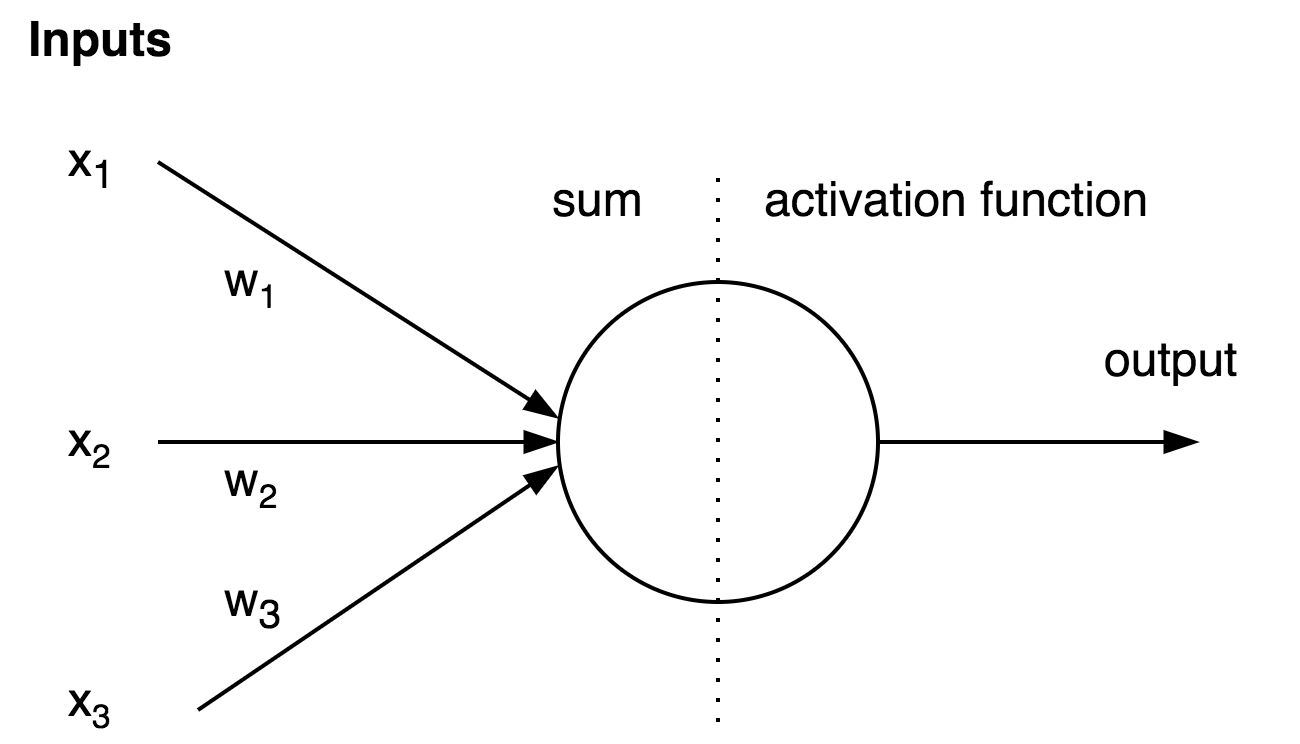
\includegraphics[width=0.3\textwidth]{perceptron}
  \caption{Model of a perceptron with three inputs.}
  \label{fig:perceptron}
\end{figure}

\newpage

This function $f$ represents the \textit{activation function}, which essentially expresses the idea that a neuron can `fire' after the sum of the inputs exceeds a certain threshold.
There are certain different functions such as the \textit{step function}, \textit{sigmoid function} and the \textit{tanh function},
which are all outlined in figure \ref{fig:activation-functions}.

\begin{figure}[ht]
  \begin{subfigure}[b]{0.32\textwidth}
    \centering
    \resizebox{\linewidth}{!}{
    \begin{tikzpicture}
      \draw[->] (-3, 0) -- (3, 0) node[right] {$x$};
      \draw[->] (-3, 0) -- (-3, 3) node[above] {$y$};
      \draw[dotted] (-3, 1.5) -- (3, 1.5);
      \draw[blue] (-3, 0) -- (0, 0);
      \draw[blue] (0, 0) -- (0, 3);
      \draw[blue] (0, 3) -- (3, 3);
    \end{tikzpicture}
    }
    \caption{The step function.}
  \end{subfigure}
  \begin{subfigure}[b]{0.32\textwidth}
    \centering
    \resizebox{\linewidth}{!}{
    \begin{tikzpicture}
      \draw[->] (-3, 0) -- (3, 0) node[right] {$x$};
      \draw[->] (-3, 0) -- (-3, 3) node[above] {$y$};
      \draw[dotted] (-3, 1.5) -- (3, 1.5);
      \draw[yscale=3,domain=-3:3,smooth,variable=\x,blue] plot ({\x},{1 / (1 + (e^(-\x)))});
    \end{tikzpicture}
    }
    \caption{The sigmoid function.}
  \end{subfigure}
  \begin{subfigure}[b]{0.32\textwidth}
    \centering
    \resizebox{\linewidth}{!}{
    \begin{tikzpicture}
      \draw[->] (-3, 0) -- (3, 0) node[right] {$x$};
      \draw[->] (-3, -1.5) -- (-3, 1.5) node[above] {$y$};
      \draw[yscale=1.5,domain=-3:3,smooth,variable=\x,blue] plot ({\x},{(2 / (1 + (e^(-2 * \x)))) - 1});
    \end{tikzpicture}
    }
    \caption{The tanh function.}
  \end{subfigure}
  \caption{Examples of different activation functions.}

\label{fig:activation-functions}
\end{figure}

Now to learn a function, the neuron adapts its weights $w_i$ such that it minimizes the error between the predicted and the expected output.
In order to achieve this, we need some manner of quantifying the error, called a \textit{loss function}.
The most commonly used ones are the \textit{mean squared error} ($\text{MSE} = (x - x')^2$) and \textit{absolute loss} ($\text{AL} = | x - x' |$) \cite{nielsen_2017}.
There are may other cost functions such as \textit{cross-entropy}, but they are not used very applicable to our specific use case.

To build a neural network, several of these perceptrons are connected together.
The most standard network is a \textit{multilayer perceptron}, also called a \textit{feedforward neural net}.
This specific network consists of an \textit{input layer}, one or more \textit{hidden layers} and an \textit{output layer} as can be seen in figure \ref{fig:feedforward}.
All of these layers have an arbitrary number of neurons and the connections between these neurons can only go from left to right and can never form a loop.
It is known that these kinds of networks can learn to approximate any function \cite{valiant2014learning}.

\begin{figure}[ht]
  \centering
  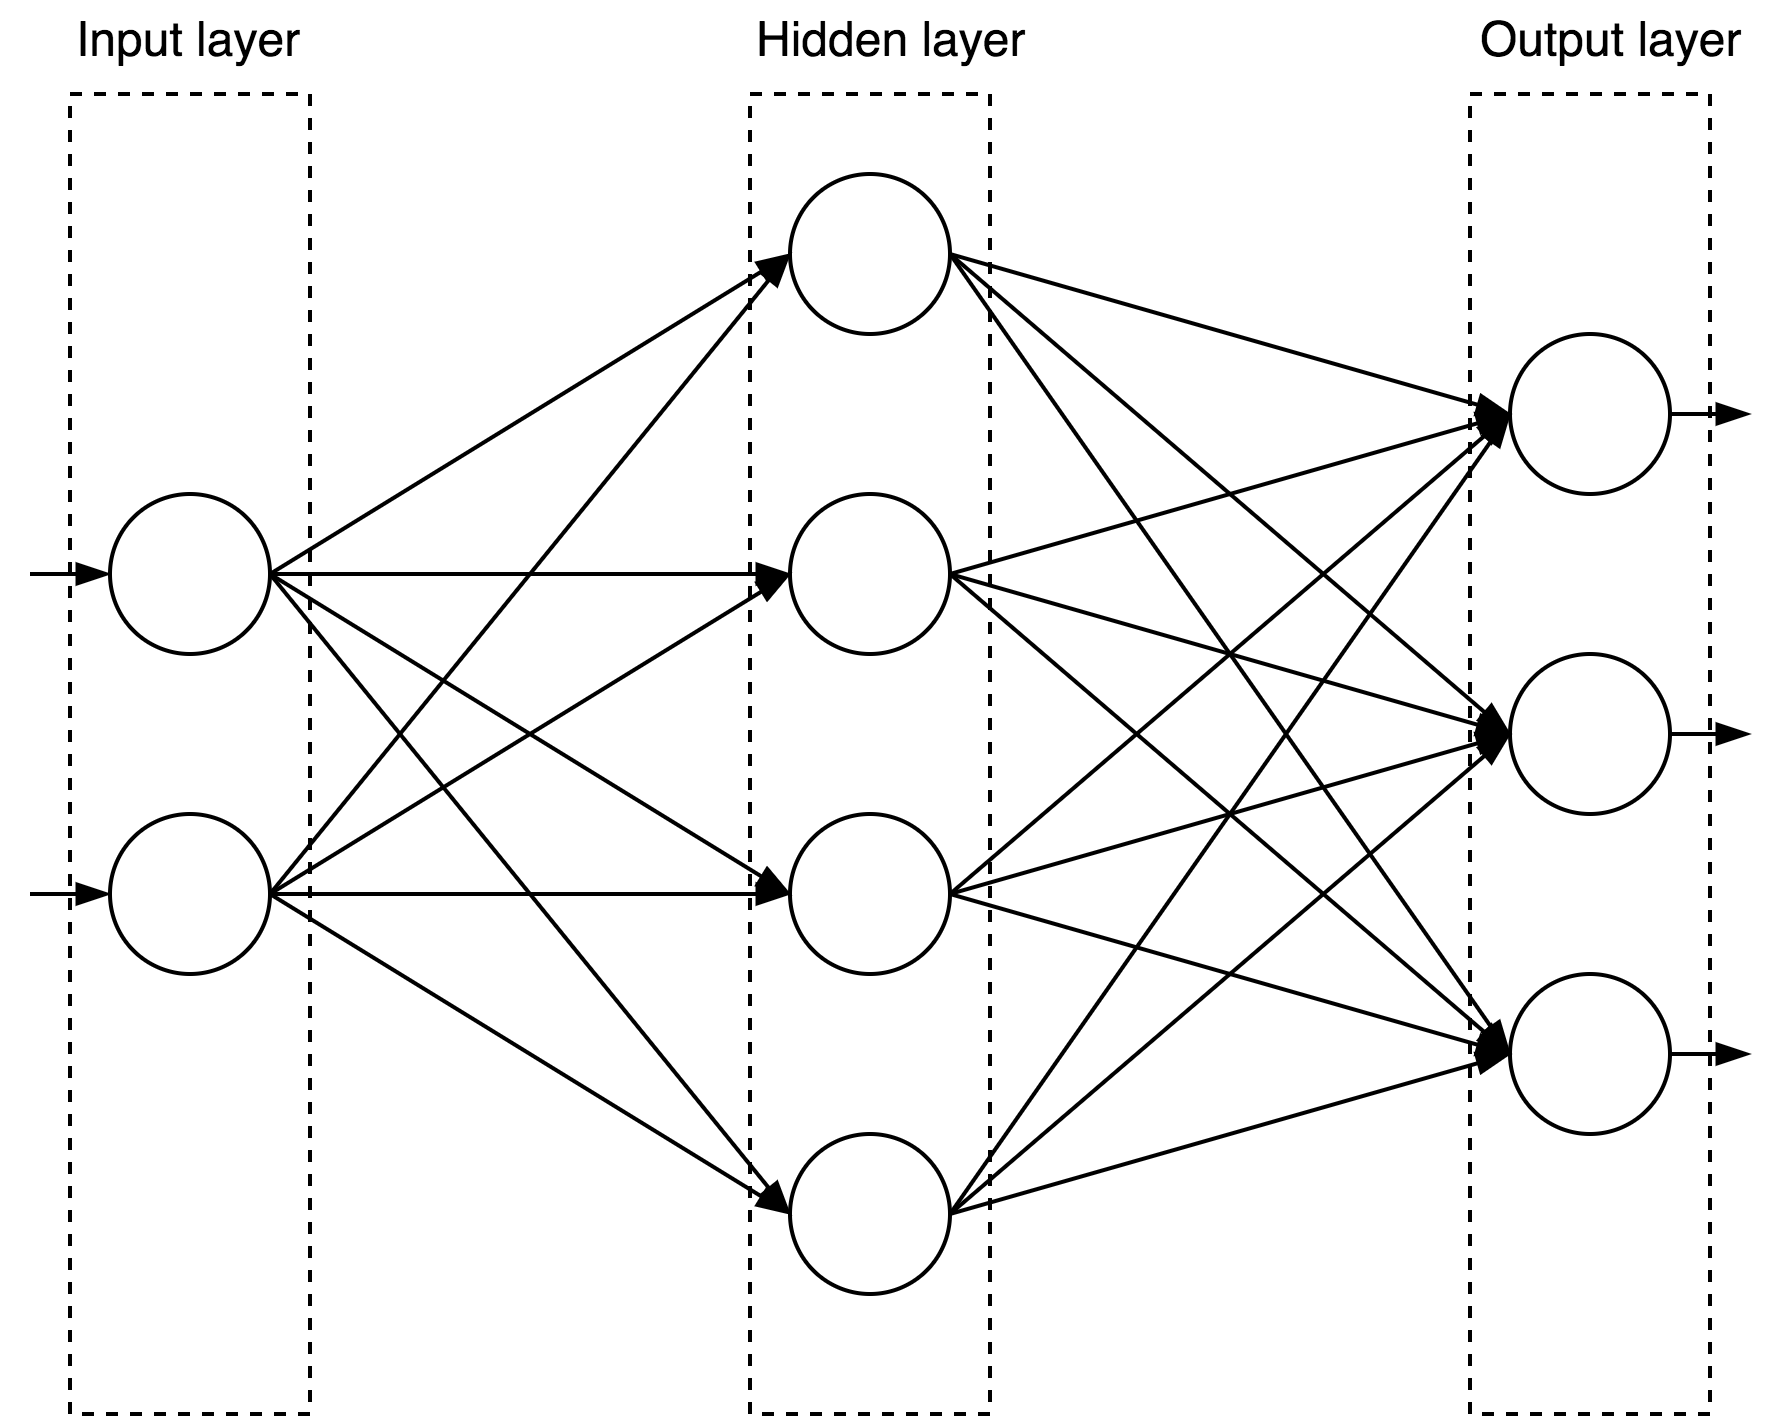
\includegraphics[width=0.6\textwidth]{feedforward}
  \caption{Example of an feedforward neural network with one hidden layer.}
  \label{fig:feedforward}
\end{figure}

Now that we know how to construct neural networks, we still need to be able to assign the appropriate weights to every connection such that the loss function is minimized.
These weights can be learned by using an algorithm, called \textit{backpropagation}.
The optimization process usually starts with initializing all of the weights with a random value and then running backpropagation.
A high level overview can be seen below \cite{nielsen_2017}:

\newpage

\begin{enumerate}
  \item Compute the outputs, given a certain input \textit{(feedforward pass)}.
  \item Calculate the error vector.
  \item Backpropagate the error by computing the differences between the expected output and the actual output, starting at the output layer and working towards the input layer.
  \item Compute the partial derivatives for the weights.
  \item Adjust the weights by subtracting these derivatives, multiplied by the \textit{learning rate}.
\end{enumerate}

The learning rate is essentially a hyperparameter to the model that defines how fast the network learns.
If its value is high, the model learns quickly and if the value is low, the model learns more slowly but the learning process will be more accurate.

The propagation process is also often done in \textit{batches}, which means that the model calculates the propagations of a fixed amount of input vectors and only once this has finished, the weighs are updates such that they minimize the outputs for the entire batch.
The size of these batches is a hyperparameter of the model.

\subsection{Stacked autoencoder}

These feedforward neural nets can be used to perform feature selection by using a specific network, called an \textit{autoencoder}.
This network tries to learn the \textit{identity function} $f(x) \approx x$ when the number of neurons in the hidden layer is smaller than the ones in the input and output layers.
Hence, essentially the network is trying to learn to learn how to compress the initial feature vector \cite{autoencoders}.

\begin{figure}[ht]
  \centering
  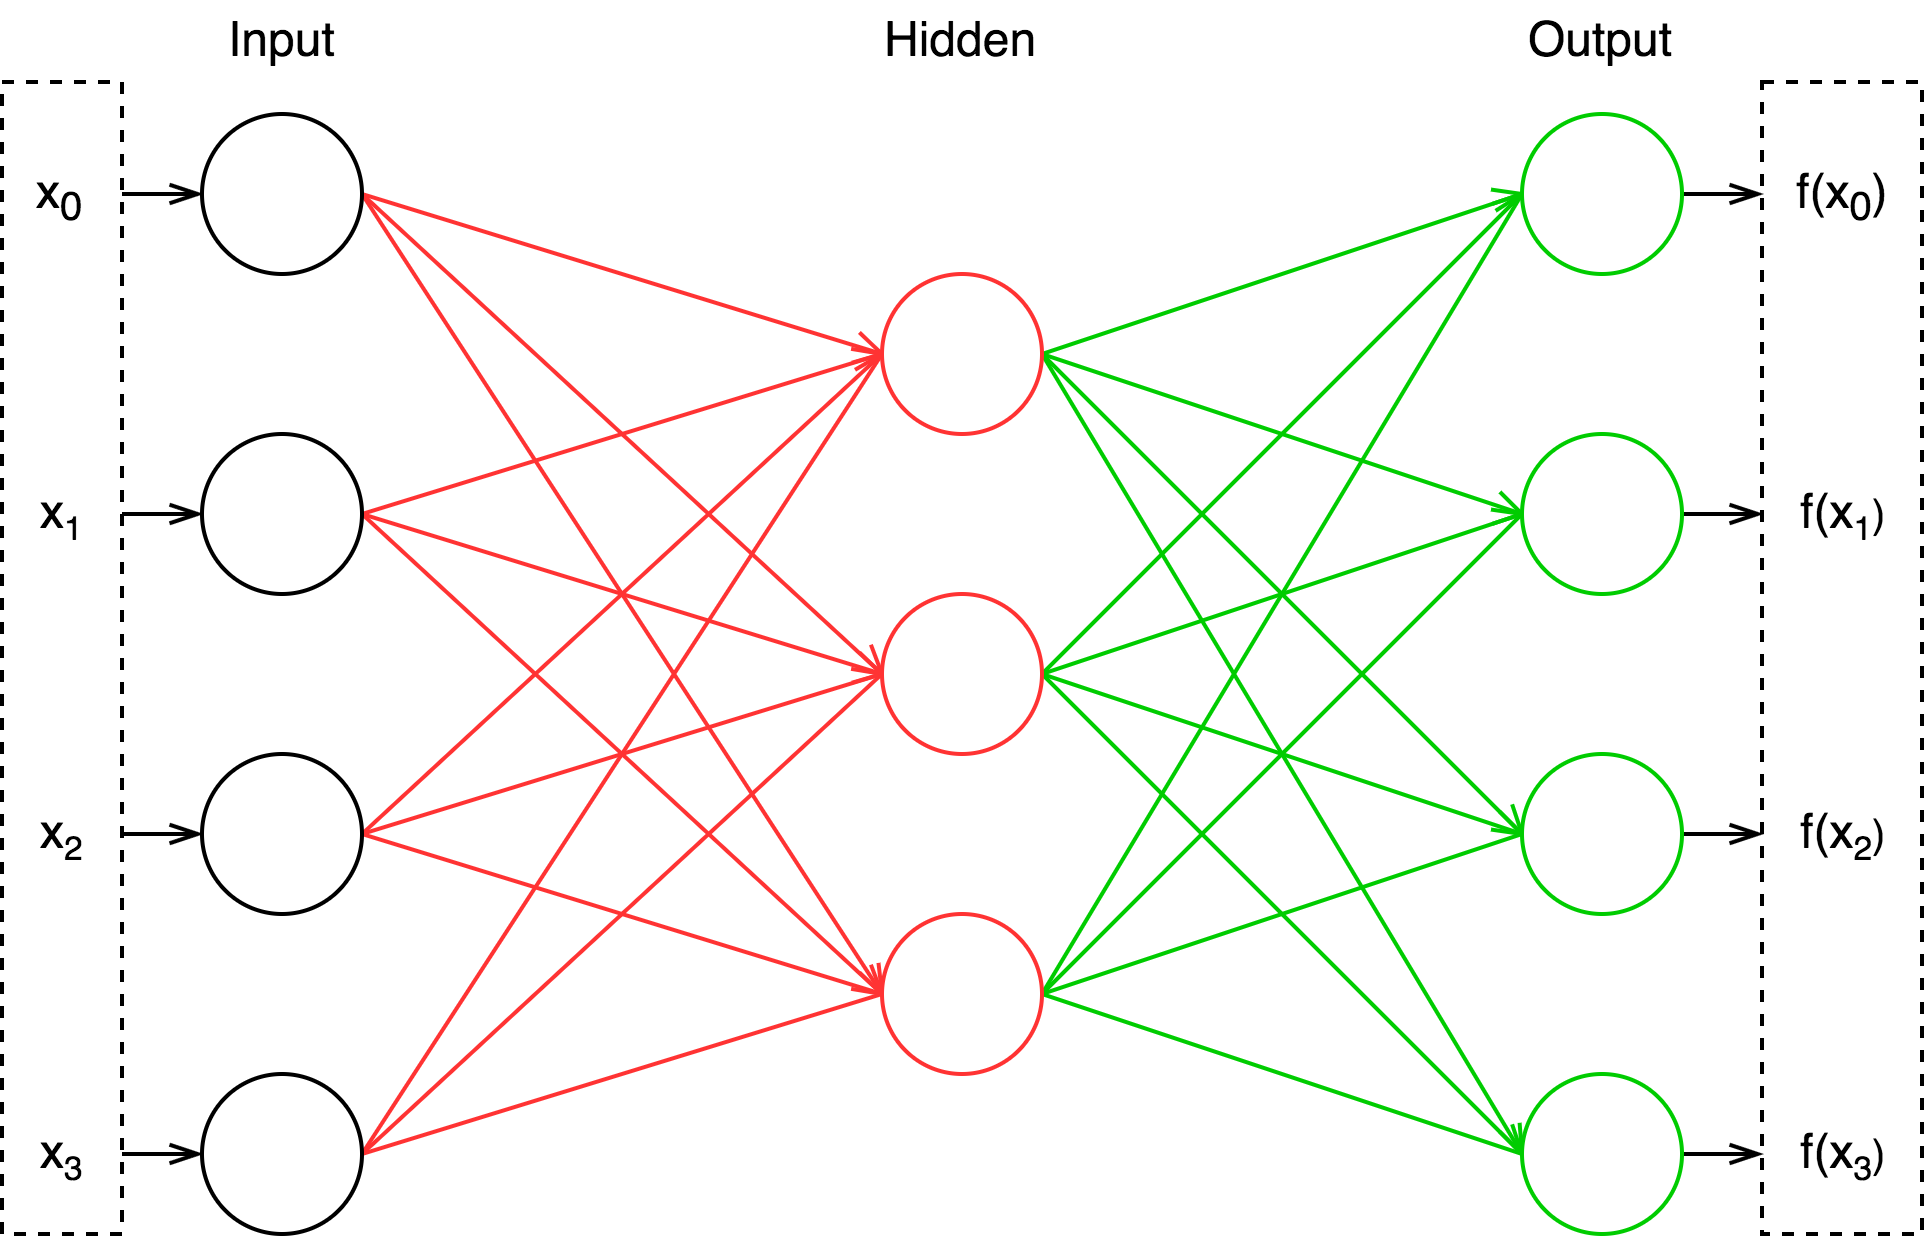
\includegraphics[width=0.6\textwidth]{autoencoder}
  \caption{Structure of a simple autoencoder.}
  \label{fig:autoencoder}
\end{figure}

In order to learn an even more compressed representation of the input, multiple layers can be introduced, where each hidden layer contains even less nodes than the previous one.
However, the problem with this approach is that the deeper the network, the more difficult it can be to learn the appropriate weights \cite{nielsen_2017}.
A solution to this problem is a greedy approach where each layer is trained in turn and then stacked on top of each other.
By this we mean that we first train the first layer, just as before.
Next, the weights of the first layer are used to transform the raw input in a compressed representation.
This representation is then used to train the second layer and so on.

\begin{figure}[ht]
  \centering
  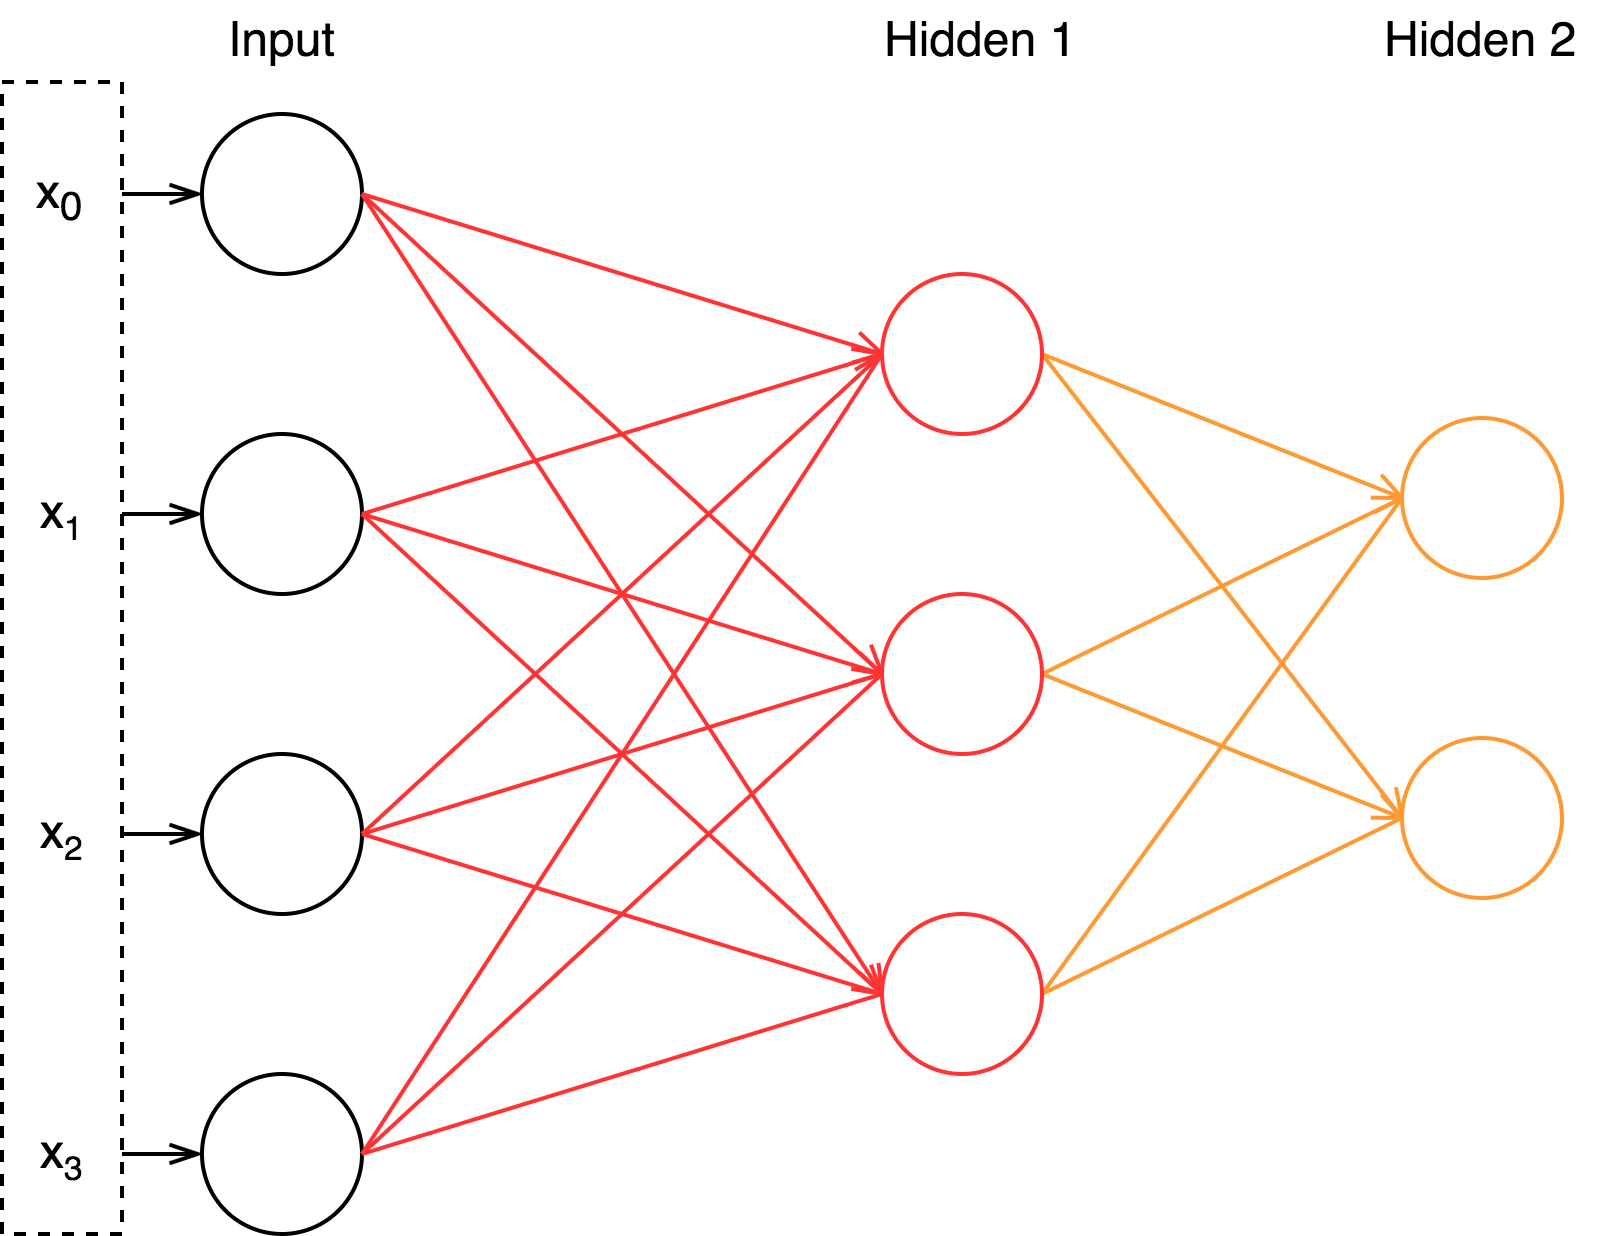
\includegraphics[width=0.55\textwidth]{stacked_autoencoder}
  \caption{Stacked autoencoder.}
  \label{fig:stacked-autoencoder}
\end{figure}

\newpage

\subsection{Recurrent Neural Networks}

Although stacked autoencoders have successfully been used in several cases \cite{deeplearningthesis,deeplearning2}, they still have a couple of drawbacks.
First of all, they require a fixed length input, which means that sequential information will need to be preprocessed.
Next, they also assume that all of the inputs and outputs are independent of each other \cite{britz_2016} whilst this might not be the case for sequential data such as the cell traces.
Hence, we will look at \textit{recurrent neural networks} (RNNs), which relaxes some of the restrictions of a feedforward neural net.
More specifically, they allow connections to form loops.

These loops basically represent that the network can be \textit{unrolled}.
For instance, for the network in figure \ref{fig:rnn}, where each square is a neural network layer, if you have a sequence that has a length of $n$, you unroll the network for $n$ steps.
Hence, we can say that an RNN has `memory' that affects the outcome of the computation, based on previous inputs \cite{britz_2016}.
So the outputs, at every time step $t$ can be calculated as follows:
$$\textit{result}, h_t = f(h_{t - 1}, x_t)$$

\begin{figure}[ht]
  \centering
  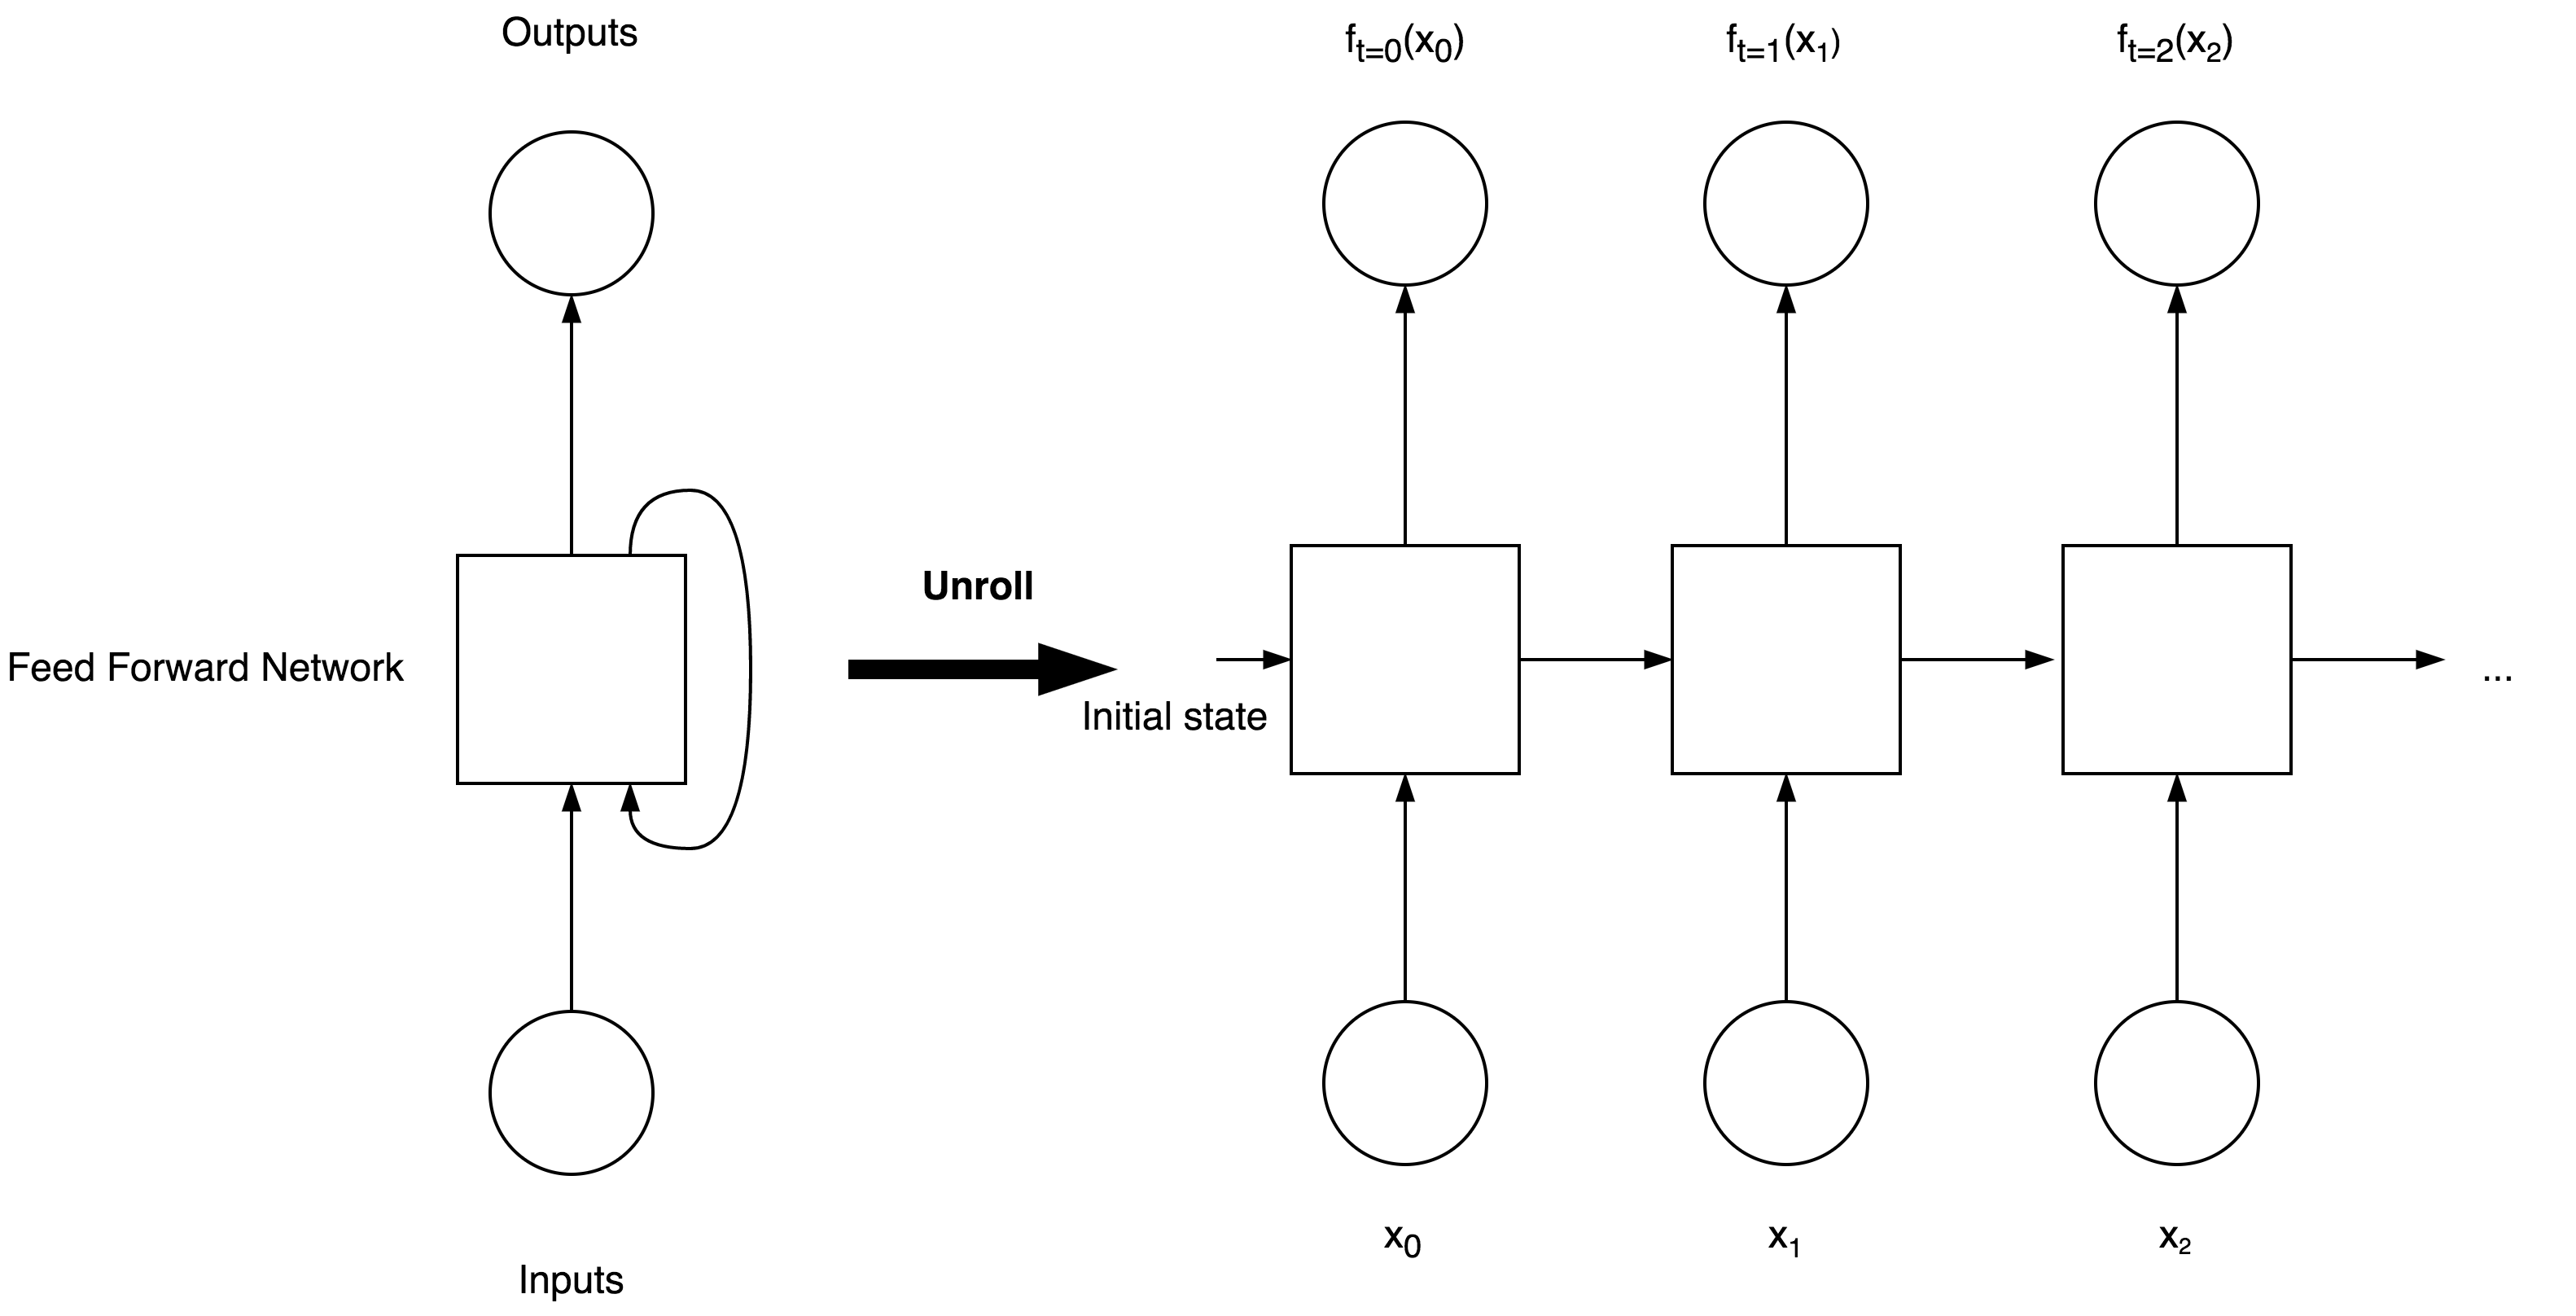
\includegraphics[width=0.90\textwidth]{rnn}
  \caption{Structure of a RNN and an example of the unrolling process \cite{britz_2016}.}
  \label{fig:rnn}
\end{figure}

Unlike traditional deep networks, every layer in the unrolled RNN shares the same weights $W$.
This greatly reduces the amount of parameters the network needs to learn \cite{britz_2016}.

One of the problems with RNNs are that they struggle to learn long-term dependencies \cite{bengio1994learning}.
So rather than using standard feedforward neural network layer at each time step, RNN cells were introduced.
Two of the most popular ones are \textit{long short-term memory} (LSTM) and \textit{gated recurring unit} (GRU) \cite{hochreiter1997long,LSTM,cho2014learning}.
Rather than just having a single neural network layer, LSTMs consist of four different layers, that all interact in a different ways \cite{LSTM}.
These interactions are outlined in figure \ref{fig:lstm}.
Although a full description is outside the scope of this paper, the general idea is based on the fact that the top state remains relatively unchanged and can therefore store long-term dependencies.
Whilst the bottom state contains more short-term information \cite{LSTM,hochreiter1997long}.

The \textit{gated recurring unit} (GRU) is a slightly more simple version of a LSTM.
The cell combines several of the gates and states to minimize the amount of parameters the model needs to learn.
Therefore, GRU allows a model to learn at a faster pace.
Whilst LSTM cells have a greater expressive power \cite{hochreiter1997long,LSTM,cho2014learning}.

\begin{figure}[ht]
  \centering
  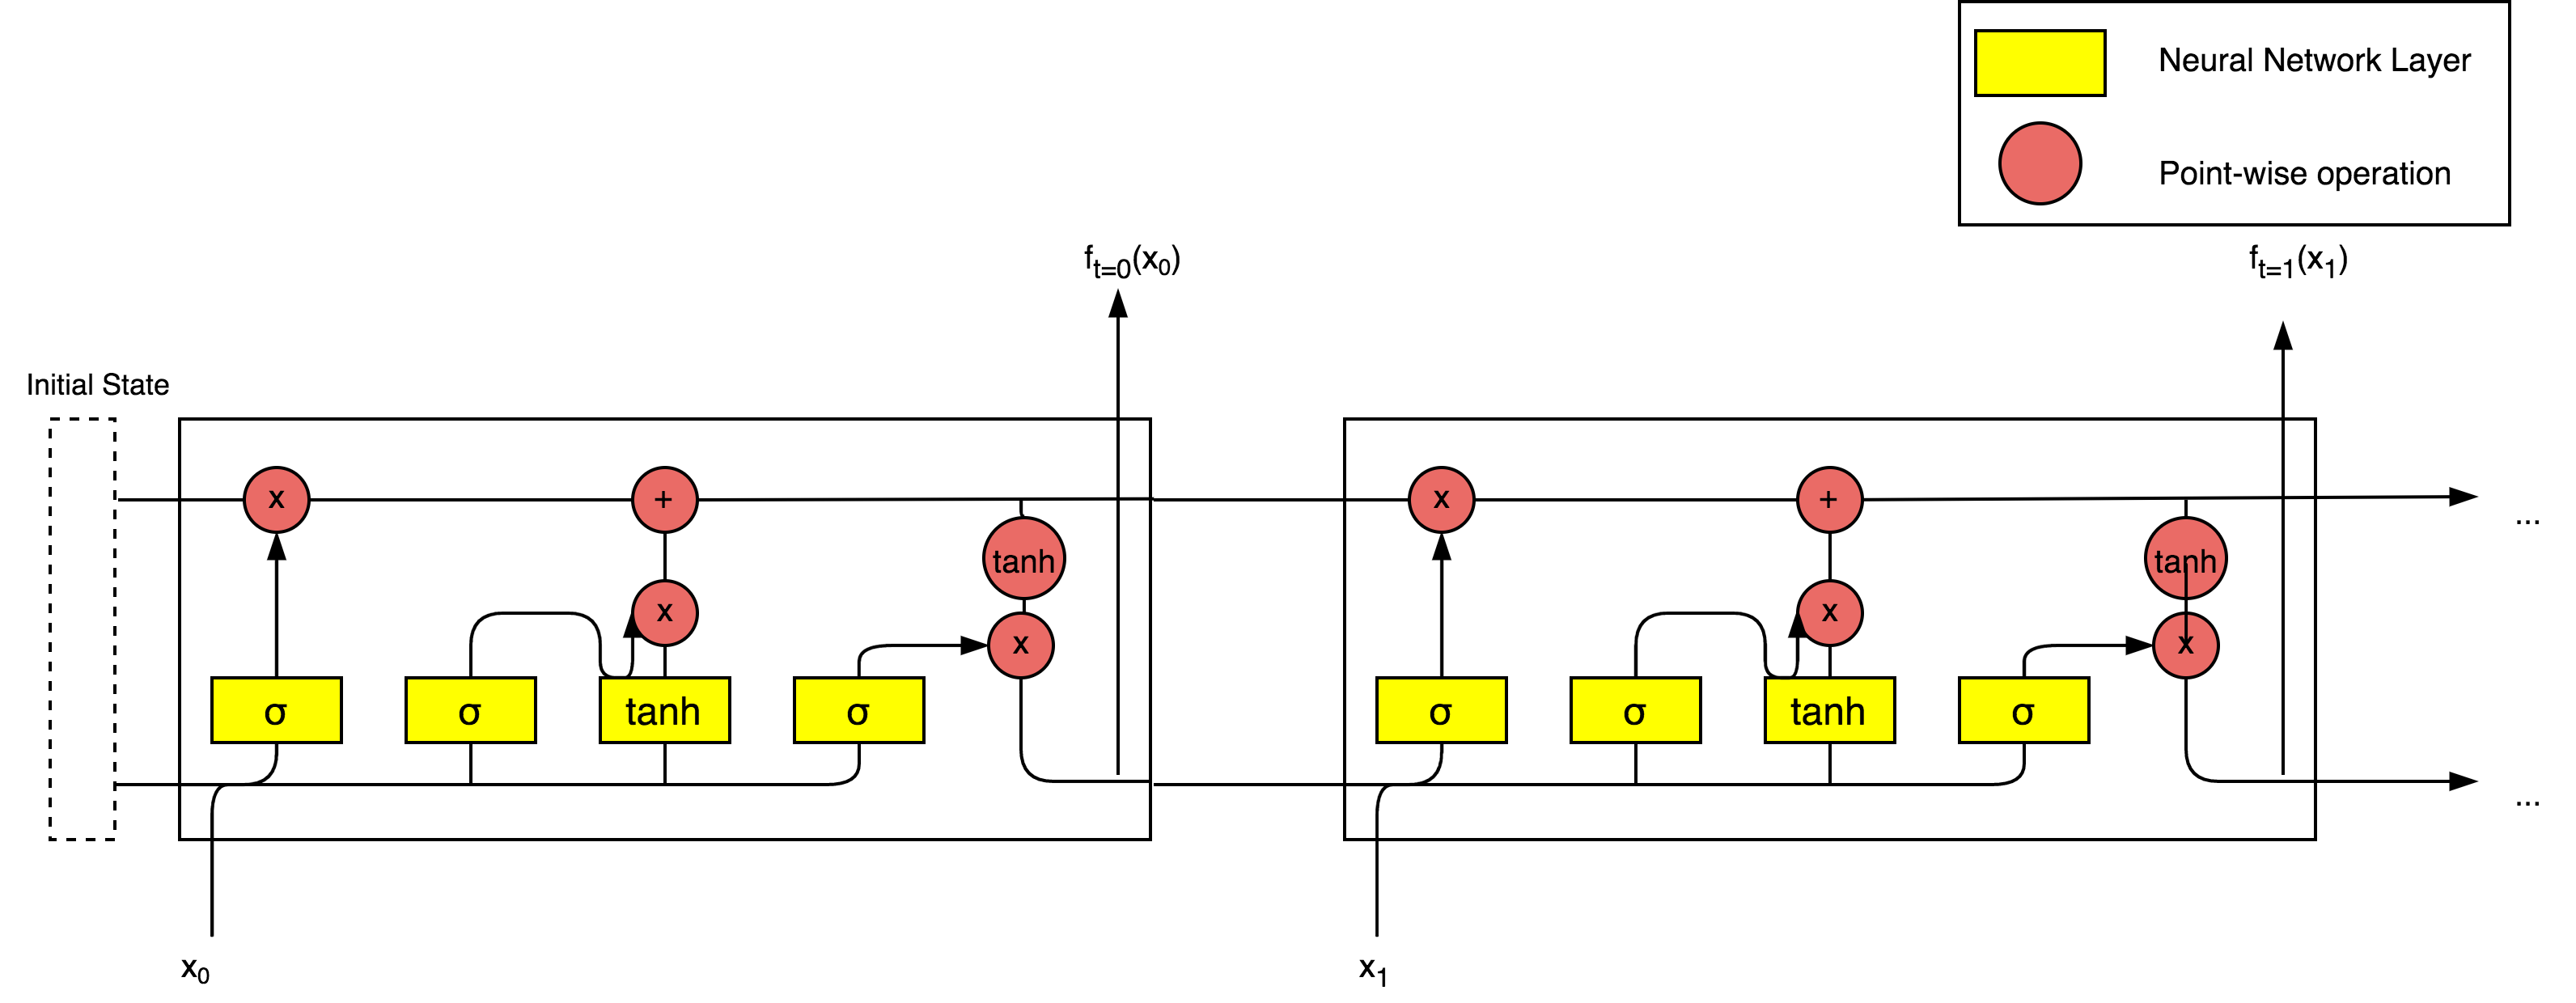
\includegraphics[width=\textwidth]{lstm}
  \caption{Interactions within a LSTM cell \cite{LSTM}.}
  \label{fig:lstm}
\end{figure}

Recurrent neural nets cannot make use of the same backpropagation algorithm used by feedforward neural nets since the unrolled layers share the same set of weights $W$.
Instead, we use a different optimization method, called \textit{backpropagation through time} (BPTT).
BPTT is similar to standard backpropagation with the key difference being that the gradients for the weights are summed at every time step $t$ \cite{britz_2016}.

\subsection{Sequence-to-Sequence Model} \label{sec:seq2seq}

One specific type of RNN, that could be used for feature generation, is a \textit{sequence-to-sequence model}.
Sometimes called a \textit{encoder-decoder model}, the model was introduced by Cho et al. \cite{cho2014learning}.
The general structure consists of two RNNs where one RNN encodes a sequence into a fixed-length representation and the other decodes those representations into another variable-length sequence \cite{cho2014learning}.
The models have been proven to be successful in several \textit{natural language processing} (NLP) tasks such as translation and response generation \cite{cho2014learning,sutskever_vinyals_le,tensorflowseq2seq}.
However, since the encoder produces a fixed-length representation, we might be able to train a sequence-to-sequence model on a copy task, just like an autoencoder, and use the \textit{thought vector} as the extracted features.

The model works as follows, each box in figure \ref{fig:seq2seq} represents an RNN cell.
We now start by unrolling the encoder, depending on the length of the input vector.
After the encoder computation is finished, the final state vector is stored in a \textit{thought vector} variable.
Next, the decoder is unrolled and run, with the though vector as its initial state and a start token as the first input.
After that, the output of the previous cell is then used as the input to the next cell until the network produces the end of sequence token \cite{cho2014learning}.
The encoder and the decoder can share the same weights or, as is more common, use a different set of parameters \cite{tensorflowseq2seq}.

\begin{figure}[ht]
  \centering
  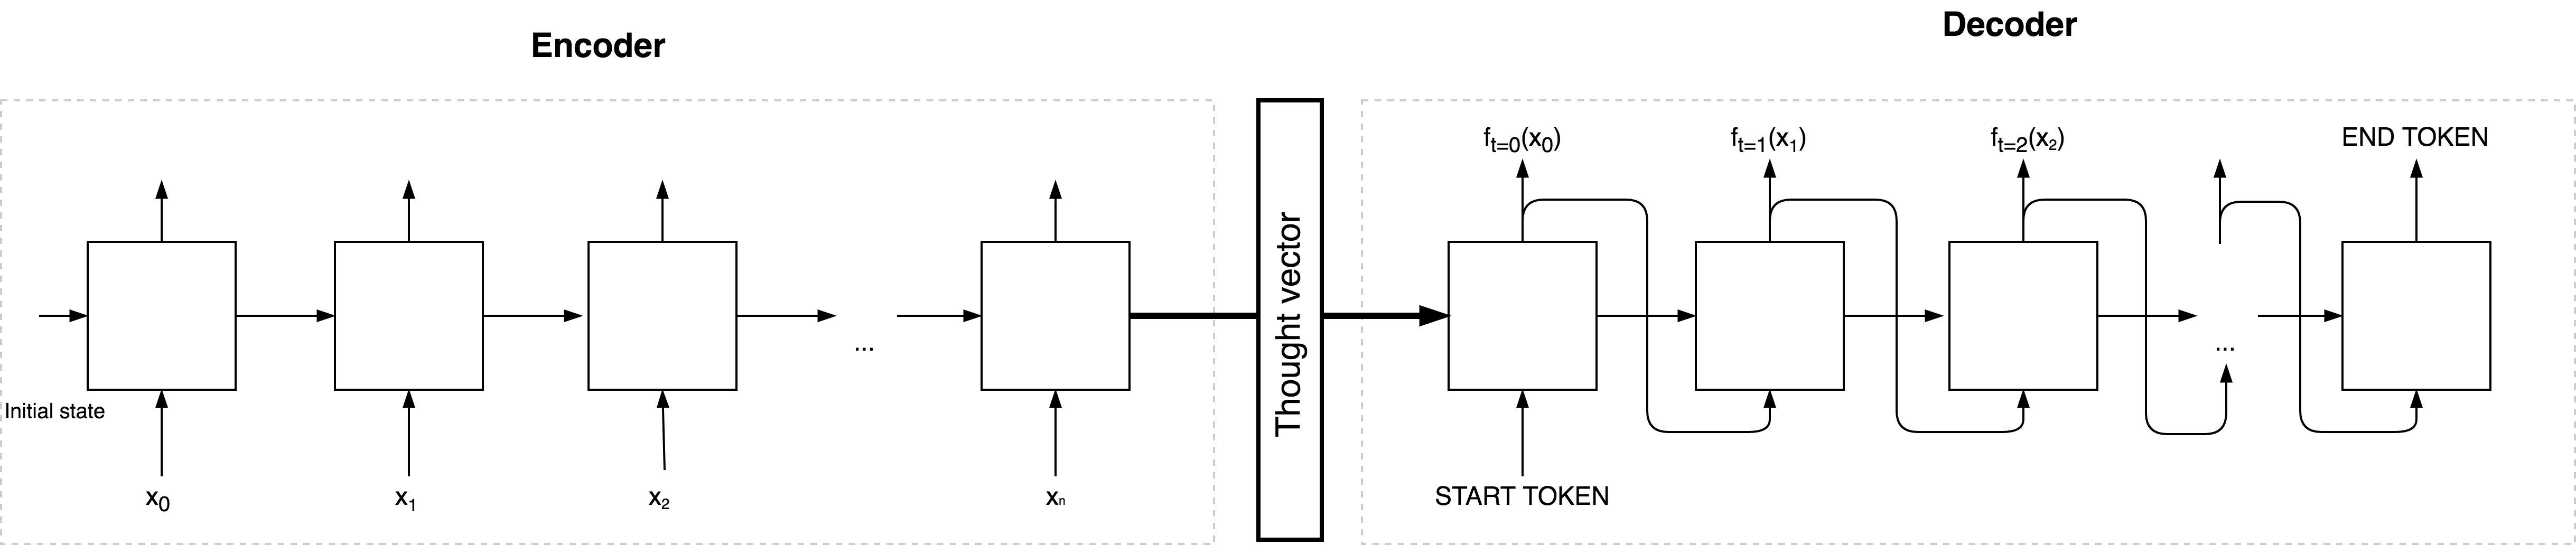
\includegraphics[width=\textwidth]{seq2seq}
  \caption{Structure of a sequence-to-sequence model \cite{britz_2016_1}.}
  \label{fig:seq2seq}
\end{figure}

If we train this model on a copy task, where it tries to reproduce the input sequence from the thought vector, it means that just like an autoencoder,
the network has learned to compress any variable-length sequence into a fixed-length representation.
So the size of the though vector is another hyperparameter to the model.

To allow a sequence-to-sequence to learn more complex representations, Sutskever et al. experimented with multilayered LSTM cells \cite{sutskever_vinyals_le}.
They showed that this model was successful in a English to French translation task and managed to cope with long-term dependencies.
Additionally, they also showed that reversing the sentences made the learning process easier.
Sutskever et al. do not have a complete explanation for this phenomenon but they believe that it is due to the many short-term dependencies in the dataset \cite{sutskever_vinyals_le}.

In addition to reversing the traces, Oshri et al. introduced the idea of using a \textit{bidirectional RNN encoder} \cite{rnnencoder}.
The idea behind this kind of encoder is based on the fact that the output at time $t$ might not only depend on past information but also on future information.
To combat this issue, the encoder consists of two layers, the forward and the backward layer, stacked on top of each other.
Next, the output is computed, based on the hidden state of both layers \cite{britz_2016}.
Finally, to extract the thought vector, the last state of both layers are extracted and averaged.

\begin{figure}[ht]
  \centering
  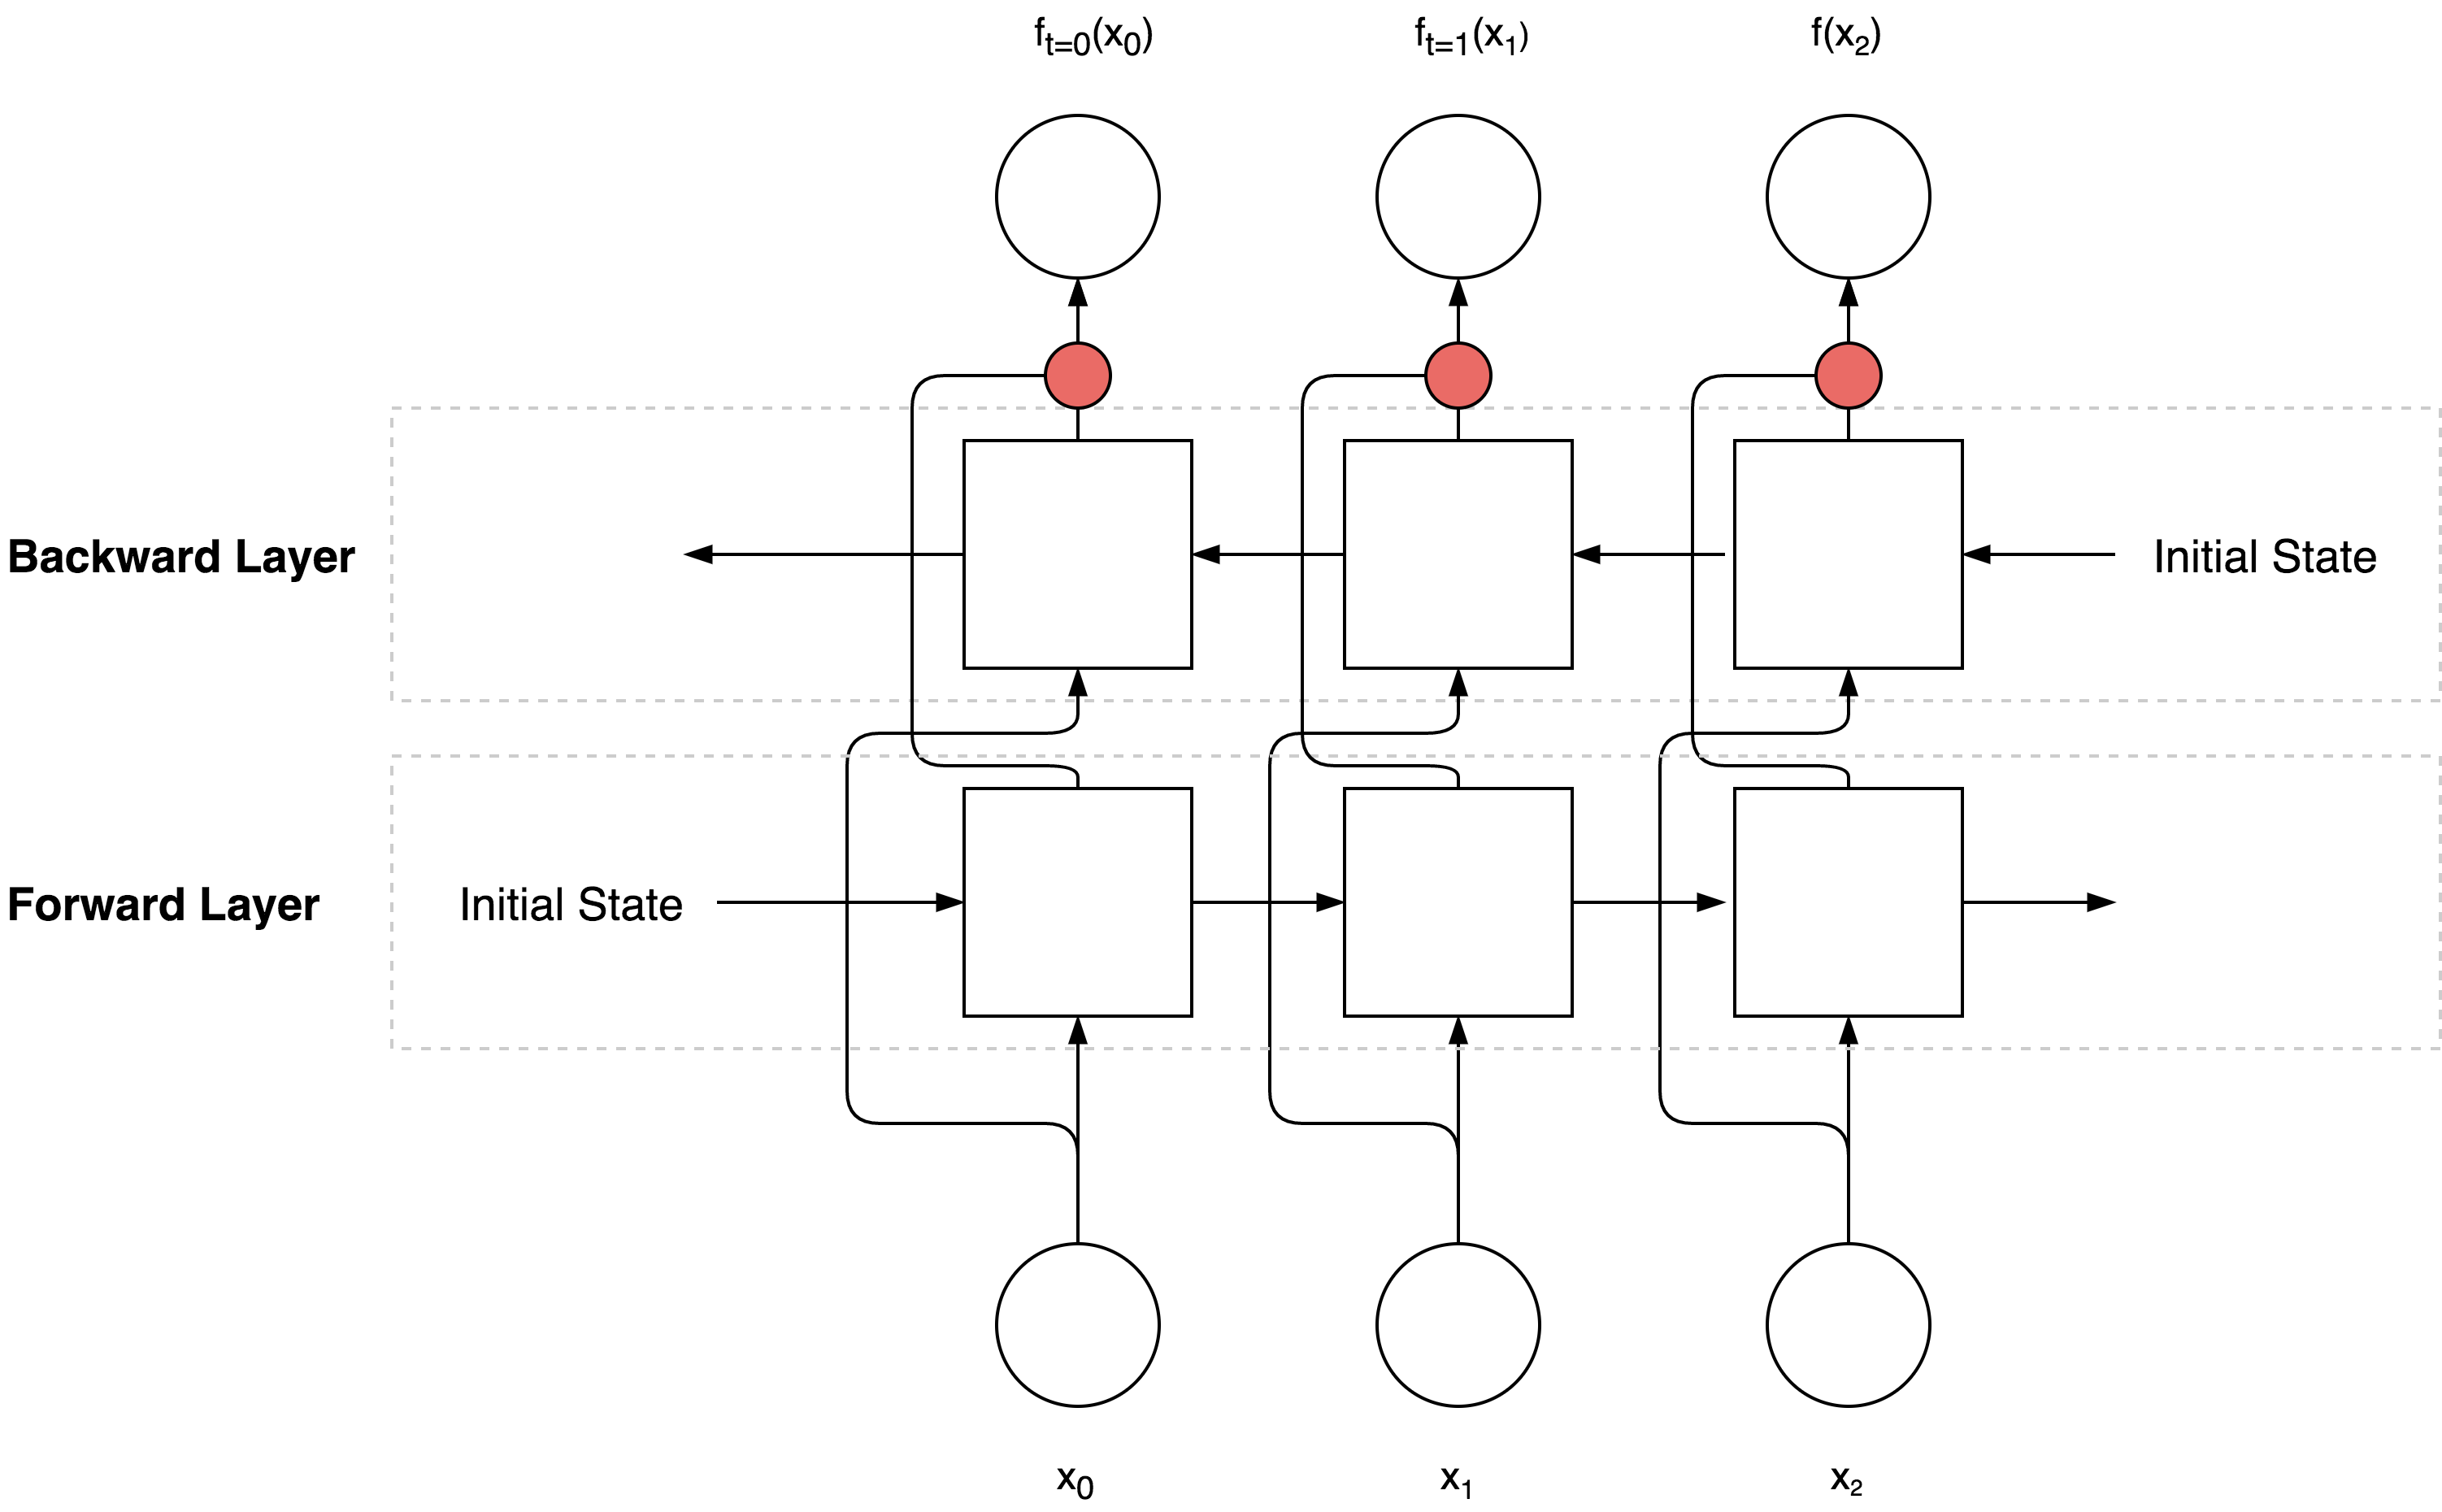
\includegraphics[width=0.9\textwidth]{bidirectional-rnn}
  \caption{Structure of a bidirectional RNN \cite{britz_2016}.}
  \label{fig:bidirectional-rnn}
\end{figure}

\newpage

This kind of model looks more appropriate than a simple sequence-to-sequence model.
However, Oshri et al. argue that the performance gain is limited, whilst introducing double the amount of parameters than a normal encoder would have \cite{rnnencoder}.

Some research by Bahdanau et al. has been to improve the performance of encoder-decoder models by introducing \textit{attention mechanisms} \cite{attention_mechanisms}.
This mechanism allows the decoder to have a more direct access to the input, thereby relieving the encoder by having to embed all the information in a fixed-length vector.
Although this technique might work well for translation tasks, our work focuses on the feature extraction process.
Therefore, we will not perform any analysis on sequence-to-sequence models with an attention mechanism.

At the time of writing, there hasn't been much research regarding using sequence-to-sequence models for feature extraction.
In fact, currently they are most often used for translation and other NLP tasks.
There they perform a classification task where the model classifies which word is likely to be next \cite{tensorflowseq2seq,cho2014learning,rnnencoder,sutskever_vinyals_le}.

% \subsection{The Vanishing Gradient Problem}
%
% Deep learning often suffers from an problem, called the \textit{vanishing gradient problem} \cite{nielsen_2017}.
% This problem represents the fact that neurons in early layers tend to learn a lot slower than those in the last layers.
% The vanishing gradient problem is also the reason why some RNNs are not able to learn long-term dependencies.
% This is due to the fact that the derivatives of both \textit{tanh} and \textit{sigmoid} activation functions approach zero near both ends.
% Thus when one of the neurons is saturated, which means that the value of the gradient gets close to zero, it drives the gradients of previous neurons to zero as well \cite{britz_2016}.
% As RNNs tend to be a lot deeper than traditional feed-forward networks, this problems tends to be a lot more common \cite{britz_2016}.
%
% \begin{figure}[ht]
%   \centering
%   \begin{subfigure}[b]{0.45\textwidth}
%     \centering
%     \resizebox{\linewidth}{!}{
%     \begin{tikzpicture}
%       \draw[->] (-3, 0) -- (3, 0) node[right] {$x$};
%       \draw[->] (-3, 0) -- (-3, 3) node[above] {$y$};
%       \draw[yscale=6,domain=-3:3,smooth,variable=\x,blue] plot ({\x},{(1 / (1 + (e^(-\x)))) * (1 - 1 / (1 + (e^(-\x))))});
%     \end{tikzpicture}
%     }
%     \caption{Derivative of the sigmoid function.}
%   \end{subfigure}
%   \begin{subfigure}[b]{0.45\textwidth}
%     \centering
%     \resizebox{\linewidth}{!}{
%     \begin{tikzpicture}
%       \draw[->] (-3, 0) -- (3, 0) node[right] {$x$};
%       \draw[->] (-3, 0) -- (-3, 3) node[above] {$y$};
%       \draw[yscale=3,domain=-3:3,smooth,variable=\x,blue] plot ({\x},{1 - ((2 / (1 + (e^(-2 * \x)))) - 1)^2});
%     \end{tikzpicture}
%     }
%     \caption{Derivative of the tanh function.}
%   \end{subfigure}
%   \caption{Derivatives of activation functions.}
% \end{figure}
%
% One solution to this problem is to use a ReLU activation function, as the derivative is either $0$ or $1$ \cite{britz_2016}.
% But both LSTM and GRU cells were especially designed to solve this issue in RNNs and therefore we will be using those throughout the rest of this paper \cite{LSTM,hochreiter1997long,cho2014learning}.

\subsection{Regularization}

Neural networks can easily \textit{overfit}.
By this we mean that the model learns noise in the training data, rather than learning to generalize.
For instance, as can be seen in figure \ref{fig:overfit}, the model generalizes when it fits a straight line but overfits otherwise.
The reason why neural nets often overfit is because of the large amount of free variables they introduce \cite{nielsen_2017}.

\begin{figure}[ht]
  \centering
  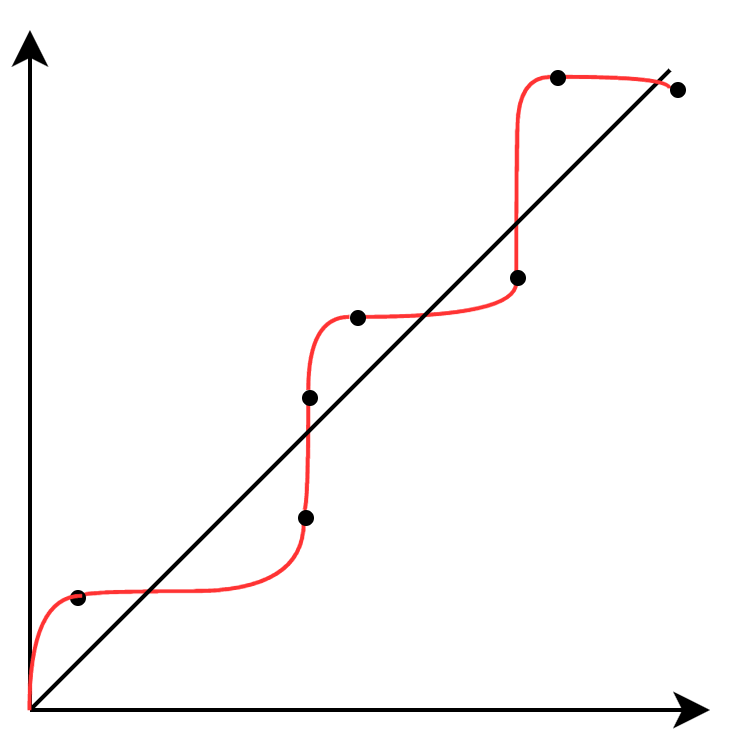
\includegraphics[width=0.3\textwidth]{overfit}
  \caption{Example of overfitting.}
  \label{fig:overfit}
\end{figure}

Overfitting can be reduced without the need to decrease the size of the network by performing \textit{regularization}.
The most popular techniques are \textit{L1}, \textit{L2}, \textit{dropout layers} and \textit{batch normalization} \cite{nielsen_2017}.
Both L1 and L2 regularization work by penalizing large weights and thus making the functions less complex.
They do this in a different fashion, for instance L1 adds the sum of the absolute values of the weights to the cost function \cite{nielsen_2017}.
Whilst L2 has a different \textit{regularization parameter}, which generally performs better than L1 in practice \cite{nielsen_2017}.

Dropout, on the other hand, doesn't modify the cost function but it changes the network.
Essentially, it ignores several neurons while performing an iteration of the backpropagation algorithm.
After that iteration, it picks a set of different neurons to ignore and repeats the process.
The effect of this is that the network basically consists of an average of various different networks.
Each of those networks will overfit in a different way so the average should reduce the total amount of overfitting \cite{nielsen_2017}.

\begin{figure}[ht]
  \centering
  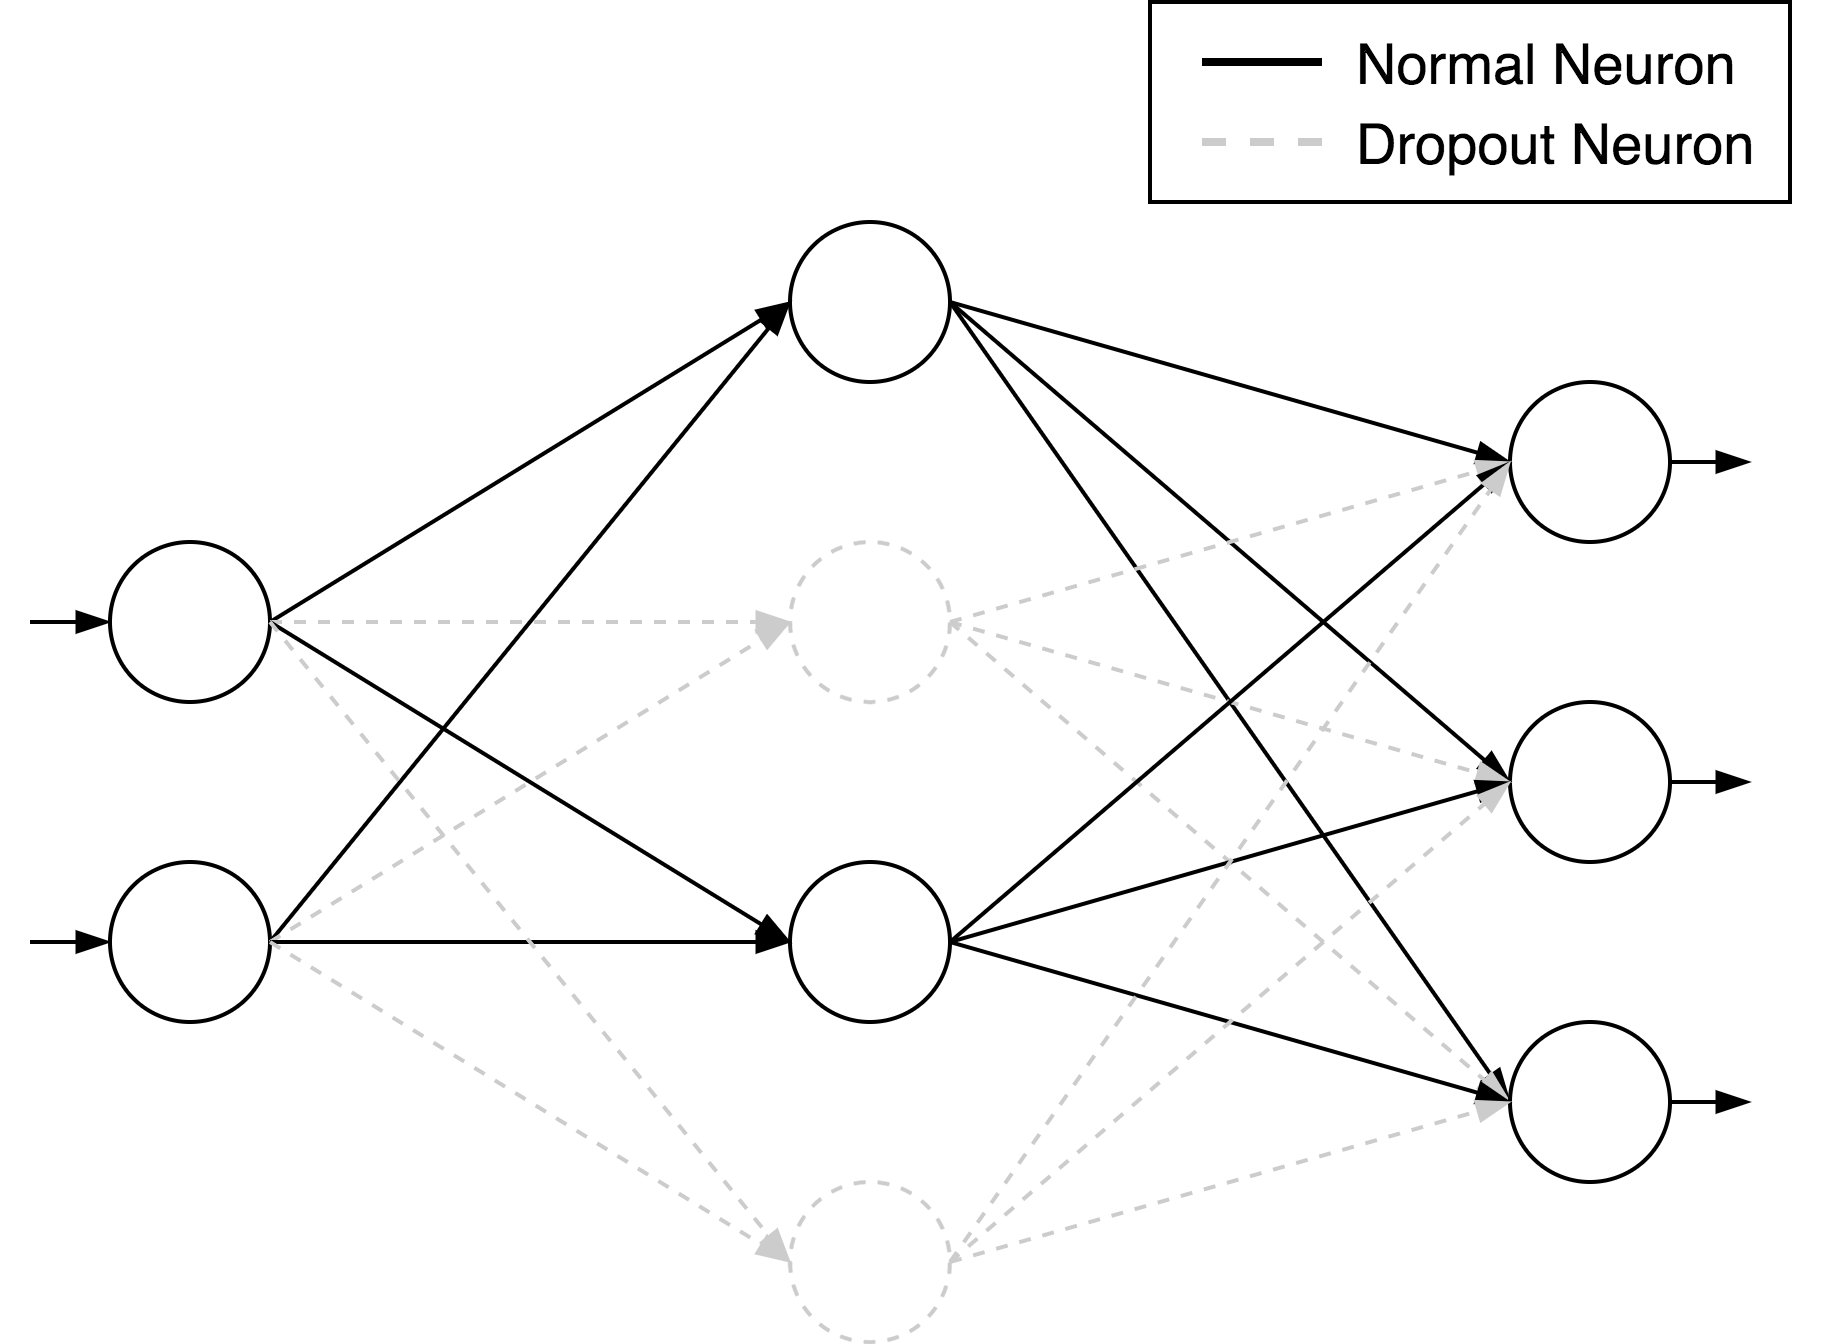
\includegraphics[width=0.6\textwidth]{dropout}
  \caption{Feedforward network with dropout.}
  \label{fig:dropout}
\end{figure}


Finally, batch normalization is a relatively new technique that also changes the network slightly by making the normalization process part of the network and performing it for every minibatch \cite{ioffe2015batch}.
Usually this wouldn't be considered a regularization technique.
However, it has been proven that it acts as a regularizer, and sometimes eliminates the need for dropout layers \cite{ioffe2015batch}.

\newpage

\section{Software Libraries}

There are various different numerical computation libraries to efficiently implement deep learning algorithms.
The most common ones being \textit{Tensorflow}, \textit{Theano}, \textit{Keras} and \textit{Torch} \cite{tensorflow,theano,keras,torch}.
The first three all provide their API in Python, whilst torch's API is in lua but a python API, called \textit{Pytorch} has been open-sourced very recently.
All of the above allow you to use \textit{cuDNN} to perform GPU-accelerated computations.

Tensorflow has a C\texttt{++} backend and its low-level API is provides more than enough flexibility to implement the required models.
It also provides a high-level API that include different RNN cells and even a sequence-to-sequence model.
However, this model has been specifically designed for NLP tasks and therefore does not support the computations that we are trying to achieve \cite{tensorflow}.
Theano is similar to Tensorflow but it does not provide all of the same high-level tools \cite{theano}.

Keras, on the other hand, runs on top of either Tensorflow or Theano.
Hence, the library provides high-level functions to create different models, rather than the low-level APIs provided by both Tensorflow and Theano.
Although this library would allow us to quickly prototype a sequence-to-sequence model, it does not provide the low-level access that we might need in order to be able to tune certain hyperparameters \cite{keras}.
Finally, Pytorch is also an attractive option but the current release is still a beta version \cite{torch}.

After a careful analysis, Tensorflow provides us with the highest flexibility whilst still providing tools to easily perform certain calculations with their high-level API.
Hence, we will use Tensorflow to implement all of our deep learning models.
On top of Tensorflow, we will also be using sklearn, which provides us with a large amount of machine learning models to perform some of our testing, and numpy for fast data preprocessing.
Both of which were chosen since they are in python, therefore allowing easy code-reuse for different modules.

\section{Data Sets}

In order to collect the necessary data, a web crawler needs to visit a large set of web pages over Tor where the traffic is recorded for every page visited.
This web crawler can emulate user browsing or simply visit web pages in \textit{Alexa's Top 10,000}, which contains the most commonly visited pages.
Or real data can be collected from users but due to privacy concerns, this data is often hard to get by.

After a web-crawler has been set up, data is collected through a TCP dump.
This data is then often preprocessed and converted into \textit{Tor cells}.
The reason for this is because Tor pads packets to a fixed-length (512 bytes) \cite{tor_project} hence these cells are a simple representation of the traffic.
Next, probabilistic techniques are used to remove SENDMEs \cite{wang_goldberg_2013}.
After this processing, a cell looks like a list of tuples, each containing a time value and a direction, which represent whether it was an incoming or outgoing packet.

\begin{table}[ht]
\centering
  \begin{tabular}{ c | c }
    \textbf{Timestamp} & \textbf{Direction} \\ \hline
      0.0&OUT \\
      0.0630009174347&OUT \\
      0.575006008148&IN \\
      0.575006008148&IN \\
      0.691473960876&IN \\
      0.719605922699&OUT \\
  \end{tabular}
  \caption{Extract of a cell trace \cite{greschbach2016effect}}
  \label{table:cell-extract}
\end{table}

All of there individual Tor cells are then stored within different files.
The names of these files will have the following format for monitored pages \texttt{<page\_id>-<instance\_id>.cell} and \texttt{<page\_id>.cell} for unmonitored pages.

There are several data sets readily available that have already been preprocessed.
Some of the largest ones are the ones collected by Wang et al. \cite{wang_cai_johnson_nithyanand_goldberg_2014} and Greschbach et al. \cite{greschbach2016effect}.
Wang et al's dataset contain traces for a $100$ monitored websites with $90$ instances each and $8400$ unmonitored sites, all from Alexa's top 10,000.
Greschbach et al. collected an even larger dataset with $100$ samples of each website in Alexa's top $9,000$ and one sample for $909,000$ unmonitored sites \cite{greschbach2016effect}.
Both of these datasets are definitely large enough to train our deep learning models.
